\documentclass[a4paper,12pt]{article} 

\usepackage[unicode, pdftex]{hyperref}

%Добавляет возможность искать и копировать текст
\usepackage{cmap}

%Убирает пробел между названием таблицы/рисунка и самой таблицей/рисунком
\usepackage{caption}
\captionsetup[table]{skip= -0 cm}
\captionsetup[figure]{skip= -0 cm}

%Выравнивание названия таблиц по левому краю
%\usepackage[nooneline]{caption} 
%Размеры отступов 
\usepackage[left=20mm, top=20mm, right=20mm, bottom=20mm, footskip=10mm]{geometry}

%Рисунки
\usepackage{graphicx}
\usepackage{wrapfig} %обтекание элементов
\graphicspath{{graphs}{figures}}  % папки с картинками

%Русский язык в формулах
\usepackage{mathtext}

%  Русский язык
\usepackage[T2A]{fontenc}			
\usepackage[utf8]{inputenc}			
\usepackage[english,russian]{babel}	

%Красная строка для первого абзаца
\usepackage{indentfirst}

%Готические буквы
\usepackage{amssymb}

% Математика
\usepackage{amsmath,amsfonts,amssymb,amsthm,mathtools} 
\usepackage{wasysym}

%Цветные подписи в таблице
\usepackage[table,xcdraw]{xcolor}

\usepackage{fancyhdr} % Колонтитулы
 	\pagestyle{fancy}
 	\renewcommand{\headrulewidth}{0.3mm}  % Толщина линейки, отчеркивающей верхний колонтитул
 	%\lfoot{Нижний левый}
 	%\rfoot{Нижний правый}
 	\rhead{Белостоцкий Артмемий, Б04-006}
 	%\chead{Верхний в центре}
 	\lhead{Лабораторная работа №11.3}
 	\renewcommand{\footrulewidth}{0.3mm}
 	\cfoot{\thepage} % По умолчанию здесь номер страницы
 	
 	
%\captionsetup[table]{
%  position=above,
%  justification=raggedright,
  %labelsep=newline, % <<< label and text on different lines
%  singlelinecheck=false % <<< raggadright also when the cap%tion is shorter
                        % than a single line
%}
 	
\begin{document} 

%Титульник 
\begin{titlepage}
	\begin{center}
		\large 	МИНИСТЕРСТВО ОБРАЗОВАНИЯ И НАУКИ РОССИЙСКОЙ ФЕДЕРАЦИИ\\
				МОСКОВСКИЙ ФИЗИКО-ТЕХНИЧЕСКИЙ ИНСТИТУТ \\
				(НАЦИОНАЛЬНЫЙ ИССЛЕДОВАТЕЛЬСКИЙ ИНСТИТУТ)\\ 
				ФИЗТЕХ-ШКОЛА ЭЛЕКТРОНИКИ, ФОТОНИКИ \\
				И МОЛЕКУЛЯРНОЙ ФИЗИКИ \\
		
		
		\vspace{4.0 cm}
		Лабораторная работа № 11.1 \\
		\LARGE \textbf{Измерение контактной разности потенциалов	}
	\end{center}
	\vspace{3 cm} \large
	
	\begin{flushright}
		выполнил студент 3 курса \\
		{группы Б04-006}\\
		\textbf{Белостоцкий Артемий}\\
	\end{flushright}
	
	\vfill

	\begin{center}
	Долгопрудный, 2023 г.
	\end{center}
\end{titlepage}                                                                      

\section*{Аннотация}

В данной работе определяется контактная разность потенциалов (p-n)--перехода в полупроводниковом диоде по результатам измерений температурной зависимости.

\section*{Теоретические сведения}

\textit{Полупроводником n-типа} называется полупроводник, в который введены доноры -- атомы 5 группы, создающие <<локальные>> уровни. Эти уровни уровни располагаются в запрещенной зоне вблизи дна зоны проводимости.

\textit{Полупроводником p-типа} называется полупроводник, в который введены акцепторы -- атомы 3 группы, создающие локальные уровни вблизи верхнего края валентной зоны, которые при низких температурах оказываются пустыми. При комнатных температурах эти уровни заполняются электронами, переходящими из валентной зоны, при этом в валентной зоне возникает дырочная проводимость.
	
\begin{figure}[h!]
	\centering
	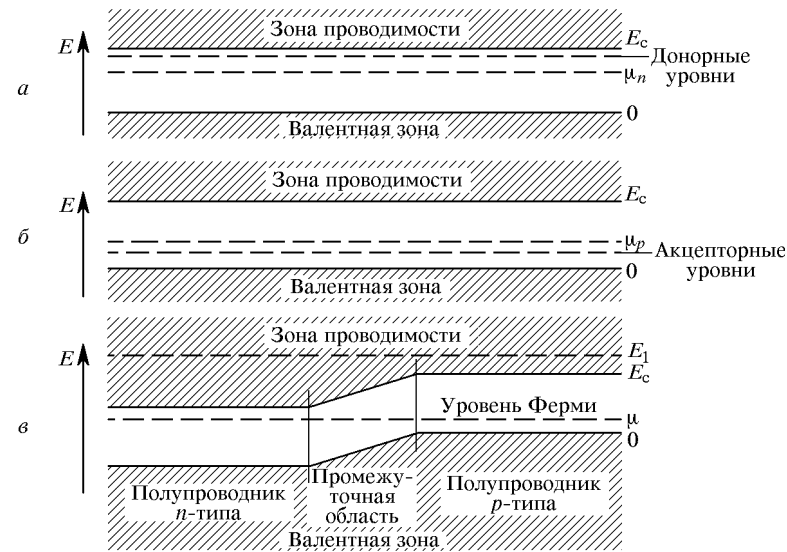
\includegraphics[width=0.8\linewidth]{semiconductor_energy}
	\caption{Энергетическая схема полупроводника: а)n-типа; б)p-типа; в) (p--n)-перехода, находящегося в равновесии}
\end{figure}

	
Приведем полупроводники n- и p- типа в соприкосновение друг с другом. В момент установления контакта происходит встречная диффузия основных носителей тока через пограничный слой; при этом дырки и электроны рекомбинируют друг с другом.

Вблизи перехода в n-области положительные ионы донорной примеси, заряд которых теперь не компенсируется электронами, образуют положительный пространственный заряд. Соответственно в p-области отрицательные ионы акцепторной примеси, заряд которых теперь не компенсируется дырками, образует отрицательный пространственный заряд. Таким образом, в области (p--n)-перехода образуется слой, обедненный носителями тока, и соответственно возникает \textit{контактная разность потенциалов} -- потенциальный барьер, препятствующий дальнейшей диффузии основных носителей.

\pagebreak

Равновесие наступает при такой высоте потенциального барьера, когда положение уровней Ферми в обеих областях совпадают. Из-за наличия потенциального барьера между концентрациями основных и неосновных носителей заряд в n- и p-областях устанавливается определенное соотношение

\begin{align*}
	\frac{n_n(n-область)}{n_n(p-область)} = \frac{n_p(n-область)}{n_p(p-область)} = \exp\left(\frac{e \Delta V}{k_Б T} \right)
\end{align*}

, где $\Delta V = \frac{k_Б T}{e} \ln \frac{n_n}{n_p}$ -- разность потенциалов в (p-n)--области

\begin{figure}[h!]
	\centering
	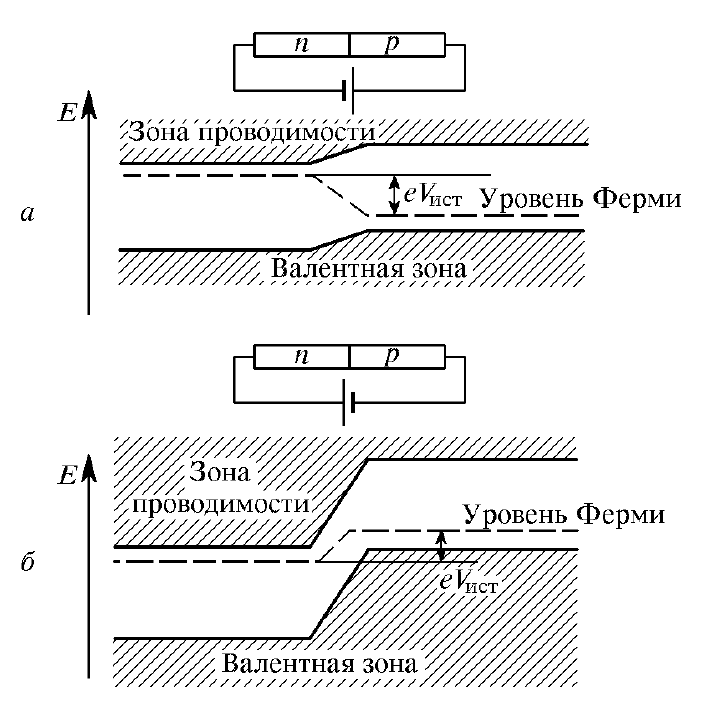
\includegraphics[width=0.7\linewidth]{external_voltage}
	\caption{Схема (p-n)--перехода под напряжением: положительное смещение (а); отрицательное смещение (б)}
\end{figure}

Приложим теперь к (p-n)--переходу напряжение $V_{ист}$ от внешнего источника тока, 	учитывая что измеряемый ток есть сумма токов дырок и электронов, получим:

\begin{align*}
	I = A \exp\left(- \frac{e \Delta V}{k_Б T}\right) \left[ \exp \left( \frac{eV_{ист}}{k_Б T}\right) - 1 \right]
\end{align*}

Заметим, что при комнатных температурах $\frac{e V_{ист}}{k_Б T} \ll 1$, тогда сопротивление перехода:

\begin{align*}
	R = \frac{V_{ист}}{I} = \frac{k_Б T}{Ae} \exp\left(\frac{e \Delta V}{k_Б T}\right) \propto \exp\left(\frac{e \Delta V}{k_Б T} \right)
\end{align*}

Тогда разность потенциалов можно найти из соотношения:

\begin{align}
	\label{eq1:delta_v}
	\Delta V = \frac{k_Б}{e} \frac{\Delta(\ln R)}{\Delta(1/T)}
\end{align}

\section*{Экспериментальная установка}

\begin{figure}[h!]
	\centering
	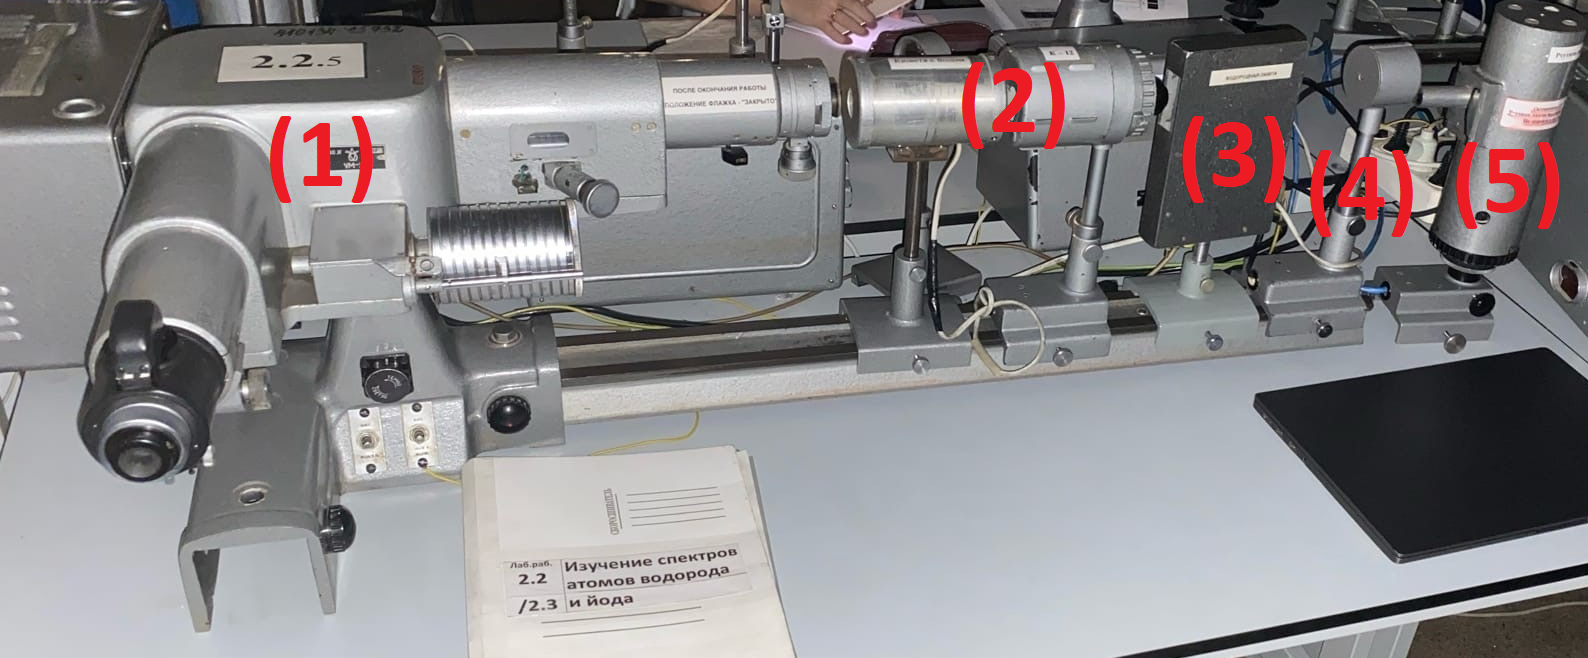
\includegraphics[width=0.8\linewidth]{setup}
	\caption{Экспериментальная установка. (1) -- осциллограф, подключенный к мосту сопротивлений, (2) -- генератор прямоугольных импульсов, (3) -- вольтметр, снимающий показания термопары, (4) -- термостат с диодом, (5) -- источник питания нагревателя, (6) -- магазин сопротивлений, (7) -- сосуд Дьюара}
\end{figure}

\begin{figure}[h!]
	\centering
	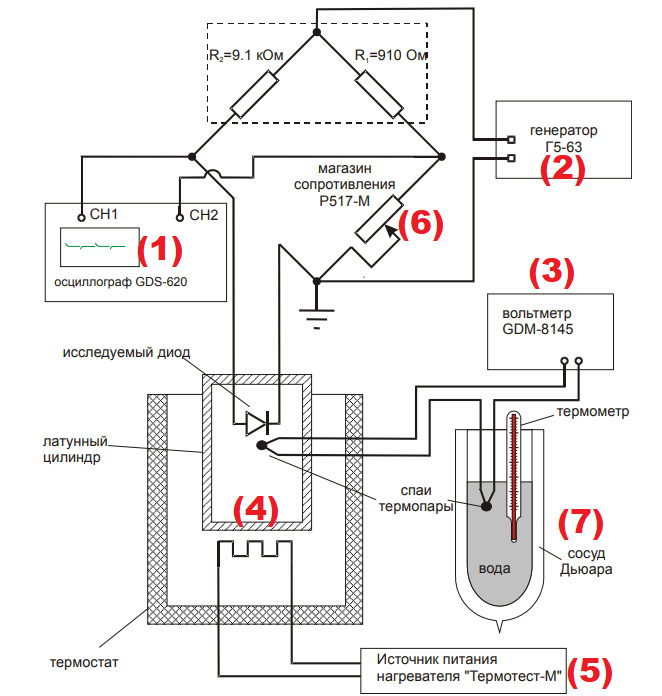
\includegraphics[width=0.7\linewidth]{scheme}
	\caption{Схема экспериментальной установки. Обозначения совпадают с обозначениями Рис.3}
\end{figure}

\newpage

\begin{figure}[h!]
	\centering
	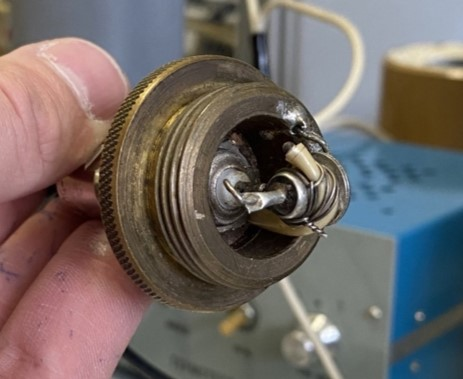
\includegraphics[width=0.7\linewidth]{diod}
	\caption{Исследуемый выпрямительный диод}
\end{figure}

Разность между температурой образца и комнатной температурой измеряется термопарой.
ЭДС термопары измеряется вольтметром, зная ЭДС можно получить температуру образца, зная постоянную термопары $\alpha = 41 \cdot 10^{-6}$ В/К

Полупроводниковый образец является одним из плеч моста сопротивлений. Мост питается от  генератора. Разность сигналов с диагонали моста видна на осциллографе. При сбалансированном (с помощью моста сопротивлений) мосте сигнал на экране осциллографа изображается в виде прямой линии, и сопротивление диода находится по формуле:

\begin{align*}
	R_д = \frac{R_2}{R_1} R_м = 10R_м
\end{align*}

\section*{Измерение контактной разности потенциалов}

Заметим, что нуль вольтметра сбит. Показания вольтметра при разнополярном подключении (без напряжения) $U_1 = -0,03$ мВ, $U_2 = -0,23$ мВ.Пусть $U_0$ истинное напряжение, тогда при подключении его к вольтметру, со сбитым на $U$ нулем, одной полярностью получим $U_0 + U$, для другой полярности $U_0 - U$. 

Следовательно, чтобы получить истинные показания вольтметра к экспериментальным точкам необходимо будет добавить величину $\sigma = -\frac{U_1 + U_2}{2} = 0,13$  мВ

Включим печь и, балансируя мост, снимем зависимость ЭДС на термопаре от сопротивления диода (оно в 10 раз больше балансирующего).

U -- показания вольтметра. При расчете T было учетно смещение нуля вольтметра, как описано выше.

\newpage

\begin{table}[h]
\centering
\caption{Зависимость температуры от сопротивление диода (нагревание)}
\begin{tabular}{|c|c|c|c|c|c|c|}
\hline
$U, мВ$ & -0,07 & 0,13 & 0,33 & 0,53 & 0,73 & 0,93 \\ \hline
$R, Ом$ & 547 & 377 & 240 & 171 & 118 & 96 \\ \hline
$R_d, Ом$ & 5470 & 3770 & 2400 & 1710 & 1180 & 960 \\ \hline
$T, K$ & 297,46 & 302,34 & 307,22 & 312,10 & 316,98 & 321,85 \\ \hline
$\ln(R_d/R_0)$ & 6,304 & 5,932 & 5,481 & 5,142 & 4,771 & 4,564 \\ \hline
$\delta_{\ln R_d/R_0}$ & 0,002 & 0,003 & 0,004 & 0,006 & 0,008 & 0,010 \\ \hline
$1/T \cdot 10^3, K^{-1}$ & 3,36 & 3,31 & 3,26 & 3,20 & 3,15 & 3,11 \\ \hline
$\delta_{1/T} \cdot 10^3, K^{-1}$ & 0,01 & 0,01 & 0,01 & 0,01 & 0,01 & 0,01 \\ \hline
\end{tabular}
\end{table}

\begin{table}[h]
\centering
\caption{Зависимость температуры от сопротивление диода (нагревание)}
\begin{tabular}{|c|c|c|c|c|c|c|}
\hline
$U, мВ$ & 1,13 & 1,34 & 1,53 & 1,73 & 1,93 & 2,06 \\ \hline
$R, Ом$ & 77 & 62 & 39 & 34 & 25 & 21 \\ \hline
$R_d, Ом$ & 770 & 620 & 390 & 340 & 250 & 210 \\ \hline
$T, K$ & 326,73 & 331
,85 & 336,49 & 341,37 & 346,24 & 349,41 \\ \hline
$\ln (R_d/R_0)$ & 4,344 & 4,127 & 3,664 & 3,526 & 3,219 & 3,045 \\ \hline
$\delta_{\ln (R_d/R_0)}$ & 0,013 & 0,016 & 0,026 & 0,029 & 0,040 & 0,048 \\ \hline
$1/T \cdot 10^3, K^{-1}$ & 3,06 & 3,01 & 2,97 & 2,93 & 2,89 & 2,86 \\ \hline
$\delta_{1/T} \cdot 10^3, K^{-1}$ & 0,01 & 0,01 & 0,01 & 0,01 & 0,01 & 0,01 \\ \hline
\end{tabular}
\end{table}

\begin{table}[h]
\centering
\caption{Зависимость температуры от сопротивление диода (охлаждение)}
\begin{tabular}{|c|c|c|c|c|c|c|c|c|c|}
\hline
$U, мВ$ & 1,99 & 1,79 & 1,59 & 1,39 & 1,19 & 0,99 & 0,79 & 0,59 & 0,39 \\ \hline
$R, Ом$ & 22 & 31 & 40 & 60 & 76 & 98 & 118 & 142 & 202 \\ \hline
$R_d, Ом$ & 220 & 310 & 400 & 600 & 760 & 980 & 1180 & 1420 & 2020 \\ \hline
$T, K$ & 347,71 & 342,83 & 337,95 & 333,07 & 328,20 & 323,32 & 318,44 & 313,56 & 308,68 \\ \hline
$\ln (R_d/R_0)$ & 3,091 & 3,434 & 3,689 & 4,094 & 4,331 & 4,585 & 4,771 & 4,956 & 5,308 \\ \hline
$\delta_{\ln (R_d/R_0)}$ & 0,045 & 0,032 & 0,025 & 0,017 & 0,013 & 0,010 & 0,008 & 0,007 & 0,005 \\ \hline
$1/T \cdot 10^3, K^{-1}$ & 2,88 & 2,92 & 2,96 & 3,00 & 3,05 & 3,09 & 3,14 & 3,19 & 3,24 \\ \hline
$\delta_{1/T} \cdot 10^3, K^{-1}$ & 0,01 & 0,01 & 0,01 & 0,01 & 0,01 & 0,01 & 0,01 & 0,01 & 0,01 \\ \hline
\end{tabular}
\end{table}

где погрешности рассчитывались по формулам:
\begin{align*}
	R_0 &= 1 Ом \\
	\delta_U &= 0,01 мВ - погрешность \ вольтметра \\
	\delta_T &= 1 K - погрешность \ термометра\\
	\delta_R &= 1 Ом - погрешность \ магазина \ сопротивлений \\
	\delta_{R_d} &= 10 \delta_R = 10 Ом \\
	\delta_T &= \sqrt{ \left( \frac{\delta_U}{\alpha} \right)^2 + \delta_{T_0}^2} = 1,03 K \\ 
	\delta_{1/T} &= \frac{\delta_T}{T^2} \\
	\delta_{\ln (R_d/R_0)} &= \frac{\delta_{R_d}}{R_d}
\end{align*}

\newpage

По полученным данным построим график зависимости $ln(R_d/R_0) = f(1/T)$

\begin{figure}[h!]
	\centering
	\includegraphics[width=0.8\linewidth]{contact_voltage}
	\caption{Зависимость $ln(R_d/R_0) = f(1/T)$. Синим отмечены точки, снятые на охлаждении, черным -- на нагревании}
\end{figure}

Аппроксимируем экспериментальные данные прямой по методу хи-квадрат:

\begin{figure}[h!]
	\centering
	\includegraphics[width=0.8\linewidth]{contact_voltage_linear}
	\caption{Зависимость $ln(R_d/R_0) = f(1/T)$, аппроксимированная прямой. Синим отмечены точки, снятые на охлаждении, черным -- на нагревании}
\end{figure}

\newpage

Тогда из аппроксимации и формулы \ref{eq1:delta_v} получим величину контактной разности потенциалов:

$$
	\Delta V \approx 0,59 В
$$

Найдем погрешность:

$$
	\delta_{\Delta V} = \frac{k_Б}{e} \delta_{\frac{\Delta(\ln R)}{\Delta(1/T)}} = 0,02  В
$$

Тогда окончательно:

$$
	\Delta V = (0,59 \pm 0,02) В
$$

\section*{Измерение ВАХ диода}

До нагревания диода было проведено измерение вольт-амперной характеристики диода. При приложении произвольного напряжения к мосту балансировка моста соответствует тому, что напряжение на диоде равно напряжению на регулируемом сопротивлении. Это позволяет выразить напряжение на диоде и ток через диод, в условиях балансировки моста, через $U_0$ -- напряжение на мосту и $R_м$ -- сопротивление моста:

\begin{align*}
	U_d &= \frac{R_м}{910 + R_м} U_0 \\
	I_d &= \frac{U_0 - U_d}{9100}
\end{align*}

Изменяя напряжение на мосту от +60 В до максимального напряжения отрицательной полярности, будем добиваться балансировки моста. Снимем значения $R_м$ и $U_0$ и по ним рассчитаем значения тока и напряжения на диоде.

\begin{table}[h]
\centering
\caption{Измерения вольт-амперной характеристики диода}
\begin{tabular}{|l|c|c|c|c|c|c|c|}
\hline
$U_0, В$ & 60 & 50 & 40 & 30 & 20 & 10 & 0 \\ \hline
$R_m, Ом$ & 476 & 489 & 499 & 508 & 518 & 528 & 0 \\ \hline
$U_d, В$ & 20,61 & 17,48 & 14,17 & 10,75 & 7,25 & 3,67 & 0 \\ \hline
$\delta_{U_d}, В$ & 0,34 & 0,35 & 0,35 & 0,36 & 0,36 & 0,37 & 0 \\ \hline
$I_d, мА$ & 4,33 & 3,57 & 2,84 & 2,12 & 1,40 & 0,70 & 0 \\ \hline
$\delta_{I_d}, мА$ &	0,12 & 0,12 & 0,12 & 0,12 & 0,12 & 0,12 & 0,11 \\ \hline
\end{tabular}
\end{table}

\begin{table}[h]
\centering
\caption{Измерения вольт-амперной характеристики диода}
\begin{tabular}{|l|l|l|l|l|l|l|l|}
\hline
$U_0, В$ & -10 & -20 & -30 & -40 & -50 & -60 & -70 \\ \hline
$R_m, Ом$ & 578 & 598 & 609 & 634 & 673 & 699 & 727 \\ \hline
$U_d, В$ & 20,61 & 17,48 & 14,17 & 10,75 & 7,25 & 3,67 & 0 \\ \hline
$\delta_{U_d}, В$ & 0,39 & 0,40 & 0,40 & 0,41 & 0,43 & 0,43 & 0,44 \\ \hline
$I_d, мА$ & -0,67 & -1,33 & -1,97 & -2,59 & -3,16 & -3,73 & -4,28 \\ \hline
$\delta_{I_d}, мА$ &	0,12 & 0,12 & 0,12 & 0,12 & 0,12 & 0,12 & 0,12 \\ \hline
\end{tabular}
\end{table}

\newpage

где погрешности определялись по формулам:

\begin{align*}
	\delta_{U_0} &= 1 В \\
	\delta_{R_м} &= 1 Ом\\
	\delta_{U_d} &= \sqrt{U_0^2 \left( \frac{1}{910 + R_м} - \frac{R_м}{(910 + R_м)^2} \right)^2 \delta^2_{R_м} + \frac{R_м}{910 + R_м} \delta^2_{U_0}} \\
	\delta_{I_d} &= \frac{\sqrt{\delta^2_{U_d} + \delta^2_{U_0}}}{9100}
\end{align*}

По полученным данным построим график зависимость $U_d = f(I_d)$ и аппроксимируем его по методу хи-квадрат зависимостью:

$$
	I_d = I_0 \left( \exp \left( \frac{eU_d}{\theta k_Б T} \right) - 1 \right)
$$

, где $\theta$ -- параметр неидеальности диода, $I_0$ -- ток насыщения.


\begin{figure}[h!]
	\centering
	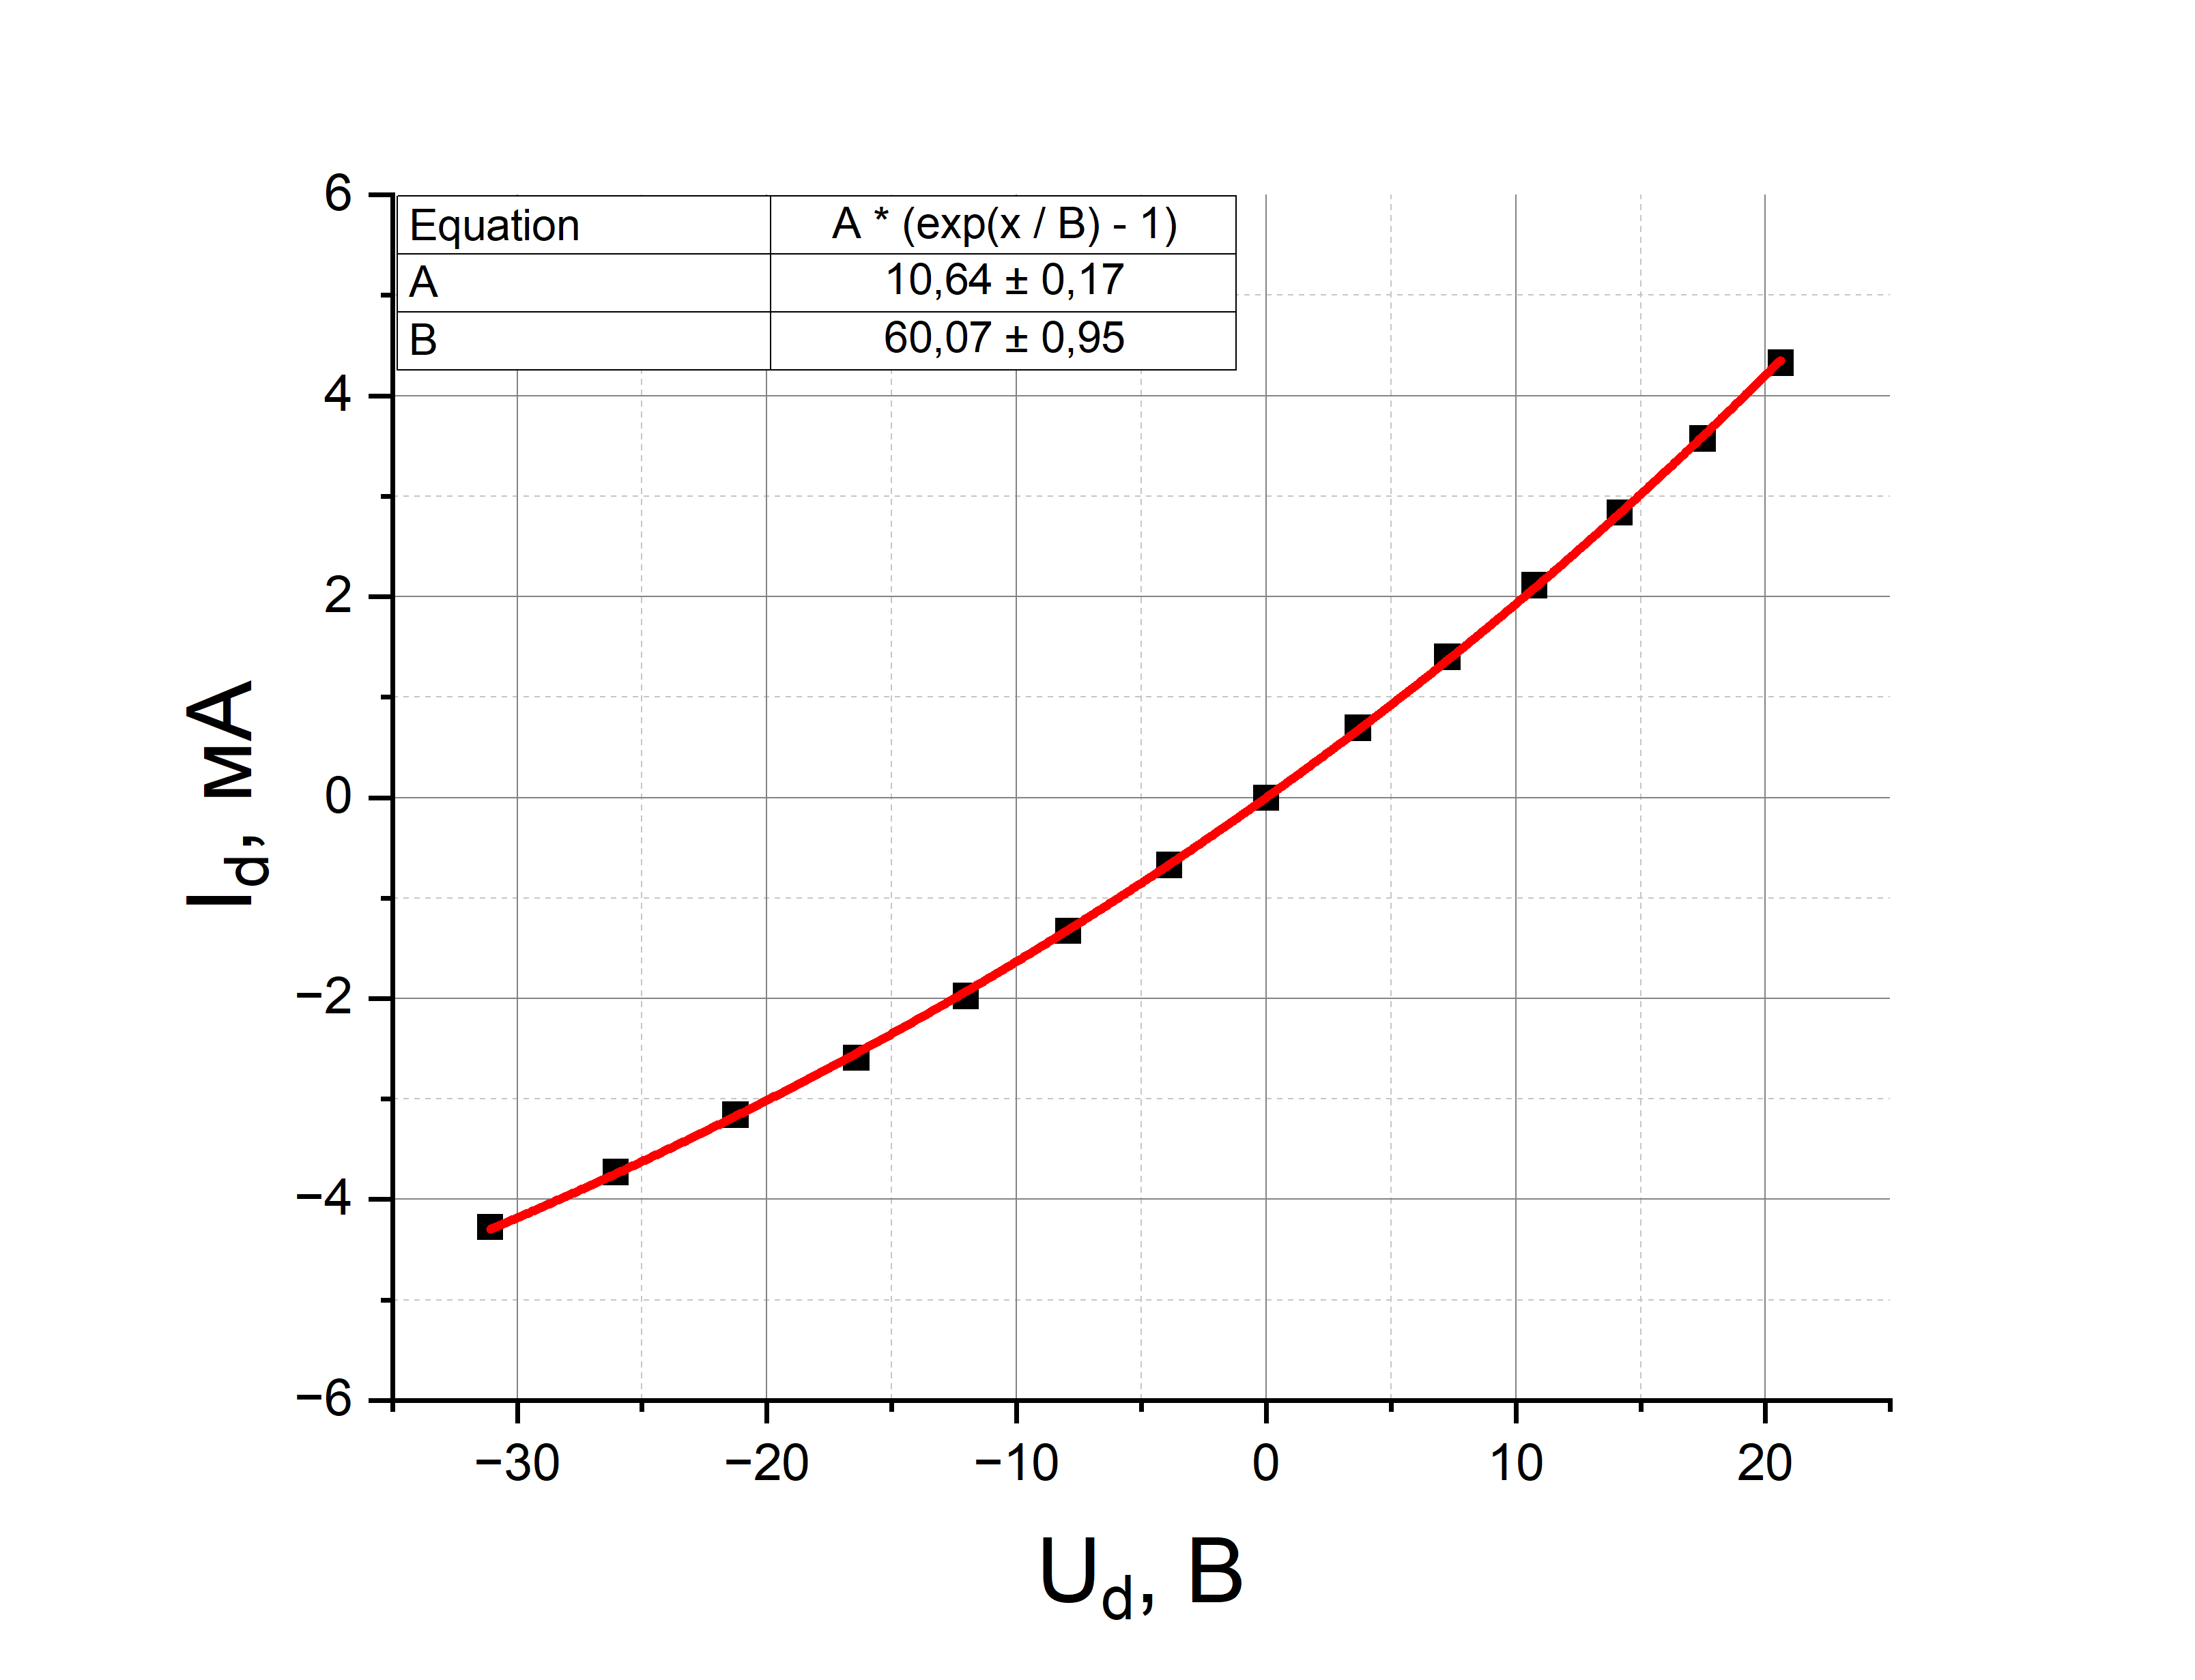
\includegraphics[width=\linewidth]{volt_amper_diod}
	\caption{Зависимость тока, протекающего через диод от напряжения на нем}
\end{figure}

Из аппроксимации получили: $I_d = (10,64 \pm 0,17) \ мА$, $\theta = 1,50 \pm 0,02$ -- что соответствует характерным параметрам выпрямительных диодов.

\newpage

\section*{Определение контактной разности потенциалов по температурной зависимости обратного тока через диод}

При приложении к диоду отрицательного напряжения большой амплитуды через диод протекает обратный ток $I_0 \propto n_n \exp(-e \Delta V / k_Б T)$. Таким образом, если измерять обратный ток при нескольких температурах, то можно определить контактную разность потенциалов. Аналогично предыдущим измерениям получим для нескольких температурах ВАХ диода, по ним определим значение обратного тока.

\begin{table}[h]
\centering
\caption{ВАХ диода при $T \approx 314 K$}
\begin{tabular}{|c|c|c|c|c|c|}
\hline
$U_0$, В & -70 & -60 & -50 & -40 & -30 \\ \hline
$R_м$, Ом & 176 & 171 & 166 & 160 & 151 \\ \hline
$U_d$, В & -11,34 & -9,49 & -7,71 & -5,98 & -4,27 \\ \hline
$\delta_{U_d}$, В & 0,17 & 0,16 & 0,16 & 0,15 & 0,14 \\ \hline
$I_d$, мА & -6,45 & -5,55 & -4,65 & -3,74 & -2,83 \\ \hline
$\delta_{I_d}$, мА & 0,11 & 0,11 & 0,11 & 0,11 & 0,11 \\ \hline
\end{tabular}
\end{table}

\begin{table}[h]
\centering
\caption{ВАХ диода при $T \approx 317 K$}
\begin{tabular}{|c|c|c|c|c|c|}
\hline
$U_0$, В & -70 & -60 & -50 & -40 & -30 \\ \hline
$R_м$, Ом & 127 & 121 & 121 & 119 & 117 \\ \hline
$U_d$, В & -8,57 & -7,04 & -5,87 & -4,63 & -3,42 \\ \hline
$\delta_{U_d}$, В & 0,14 & 0,13 & 0,12 & 0,12 & 0,12 \\ \hline
$I_d$, мА & -6,75 & -5,82 & -4,85 & -3,89 & -2,92 \\ \hline
$\delta_{I_d}$, мА & 0,11 & 0,11 & 0,11 & 0,11 & 0,11 \\ \hline
\end{tabular}
\end{table}

\begin{table}[h]
\centering
\caption{ВАХ диода при $T \approx 332 K$}
\begin{tabular}{|c|c|c|c|c|c|}
\hline
$U_0$, В & -70 & -60 & -50 & -40 & -30 \\ \hline
$R$, Ом & 63 & 62 & 61 & 61 & 60 \\ \hline
$U_d$, В & -4,53 & -3,83 & -3,14 & -2,51 & -1,86 \\ \hline
$\delta_{U_d}$, В & 0,09 & 0,09 & 0,08 & 0,07 & 0,07 \\ \hline
$I_d$, мА & -7,19 & -6,17 & -5,15 & -4,12 & -3,09 \\ \hline
$\delta_{I_d}$, мА & 0,11 & 0,11 & 0,11 & 0,11 & 0,11 \\ \hline
\end{tabular}
\end{table}

\begin{table}[h!]
\centering
\caption{ВАХ диода при $T \approx 336 K$}
\begin{tabular}{|c|c|c|c|c|c|}
\hline
$U_0$, В & -70 & -60 & -50 & -40 & -30 \\ \hline
$R$, Ом & 43 & 42 & 41 & 41 & 40 \\ \hline
$U_d$, В & -3,16 & -2,65 & -2,16 & -1,72 & -1,26 \\ \hline
$\delta_{U_d}$, В & 0,08 & 0,07 & 0,07 & 0,06 & 0,05 \\ \hline
$I_d$, мА & -7,35 & -6,30 & -5,26 & -4,21 & -3,16 \\ \hline
$\delta_{I_d}$, мА & 0,11 & 0,11 & 0,11 & 0,11 & 0,11 \\ \hline
\end{tabular}
\end{table}

Погрешности были рассчитаны по формулам из предыдущего пункта.

Аналогично предыдущему пункту аппроксимируем вольт-амперные характеристики по методу хи-квадрат, чтобы узнать значение тока насыщения -- $I_0$

\newpage

\begin{figure}[h!]
	\centering
	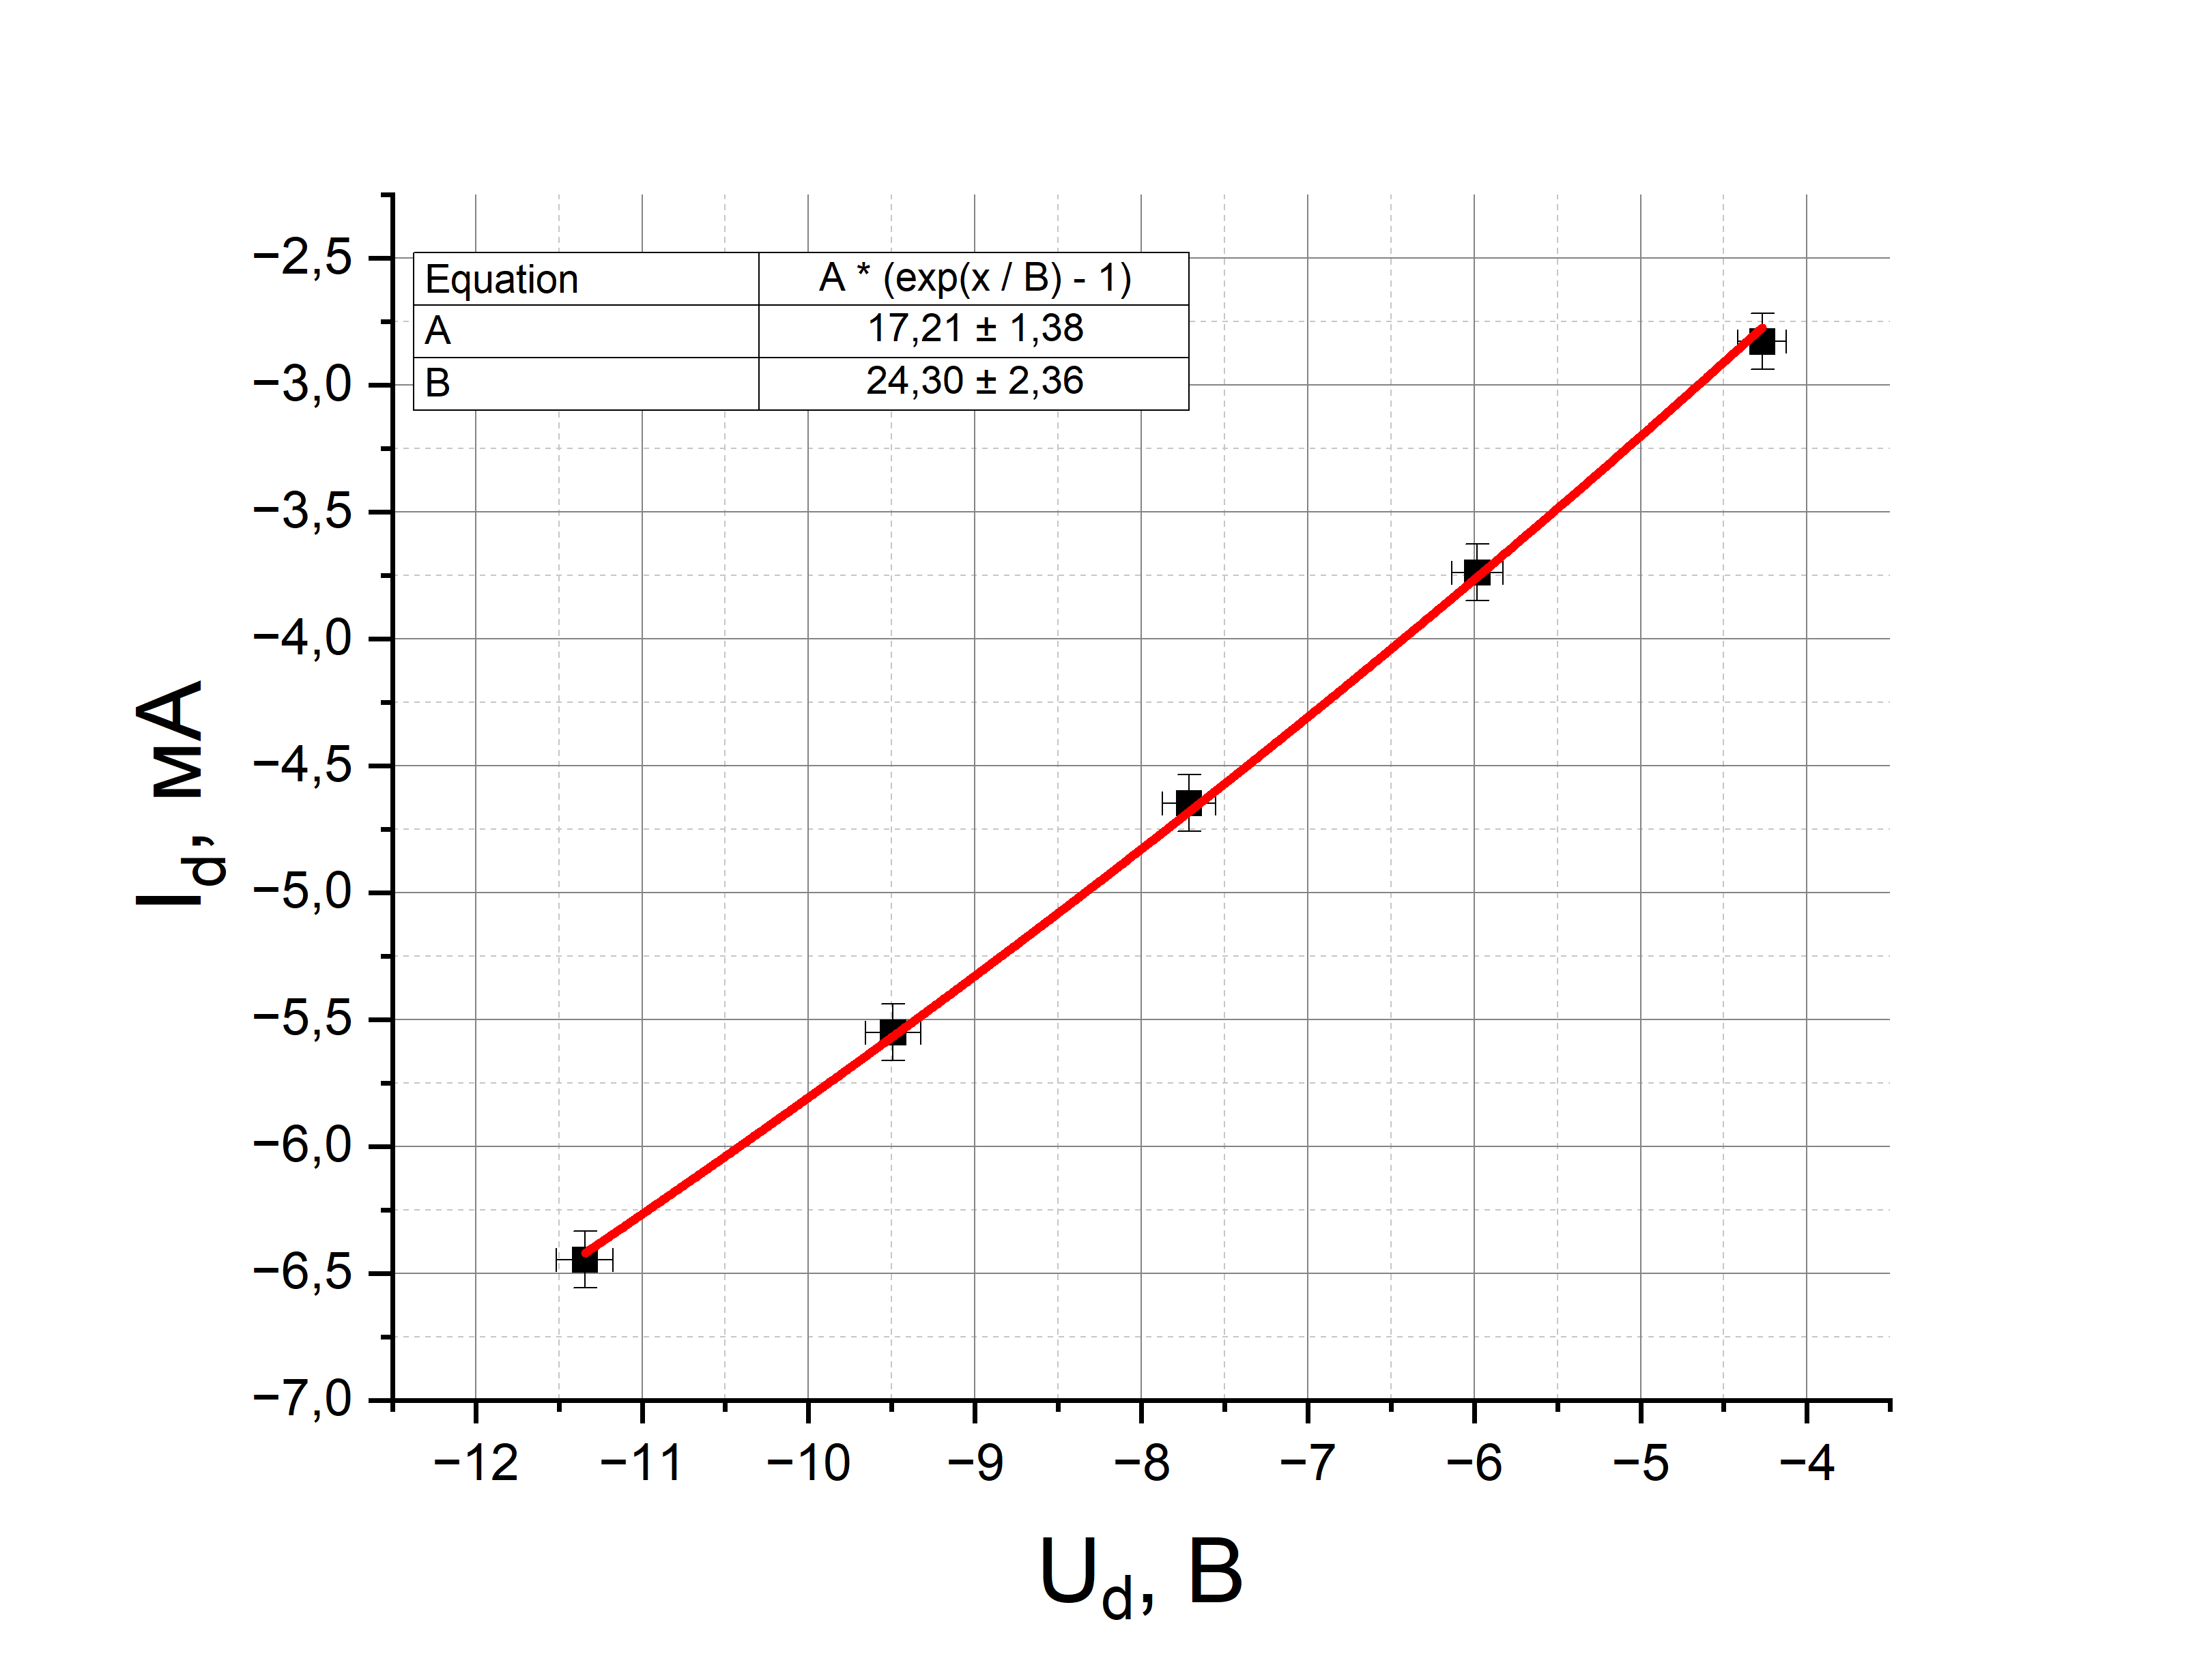
\includegraphics[width=0.8\linewidth]{reverse_T_1}
	\caption{Зависимость тока, протекающего через диод от напряжения на нем при $T \approx 314K$}
\end{figure}

\begin{figure}[h!]
	\centering
	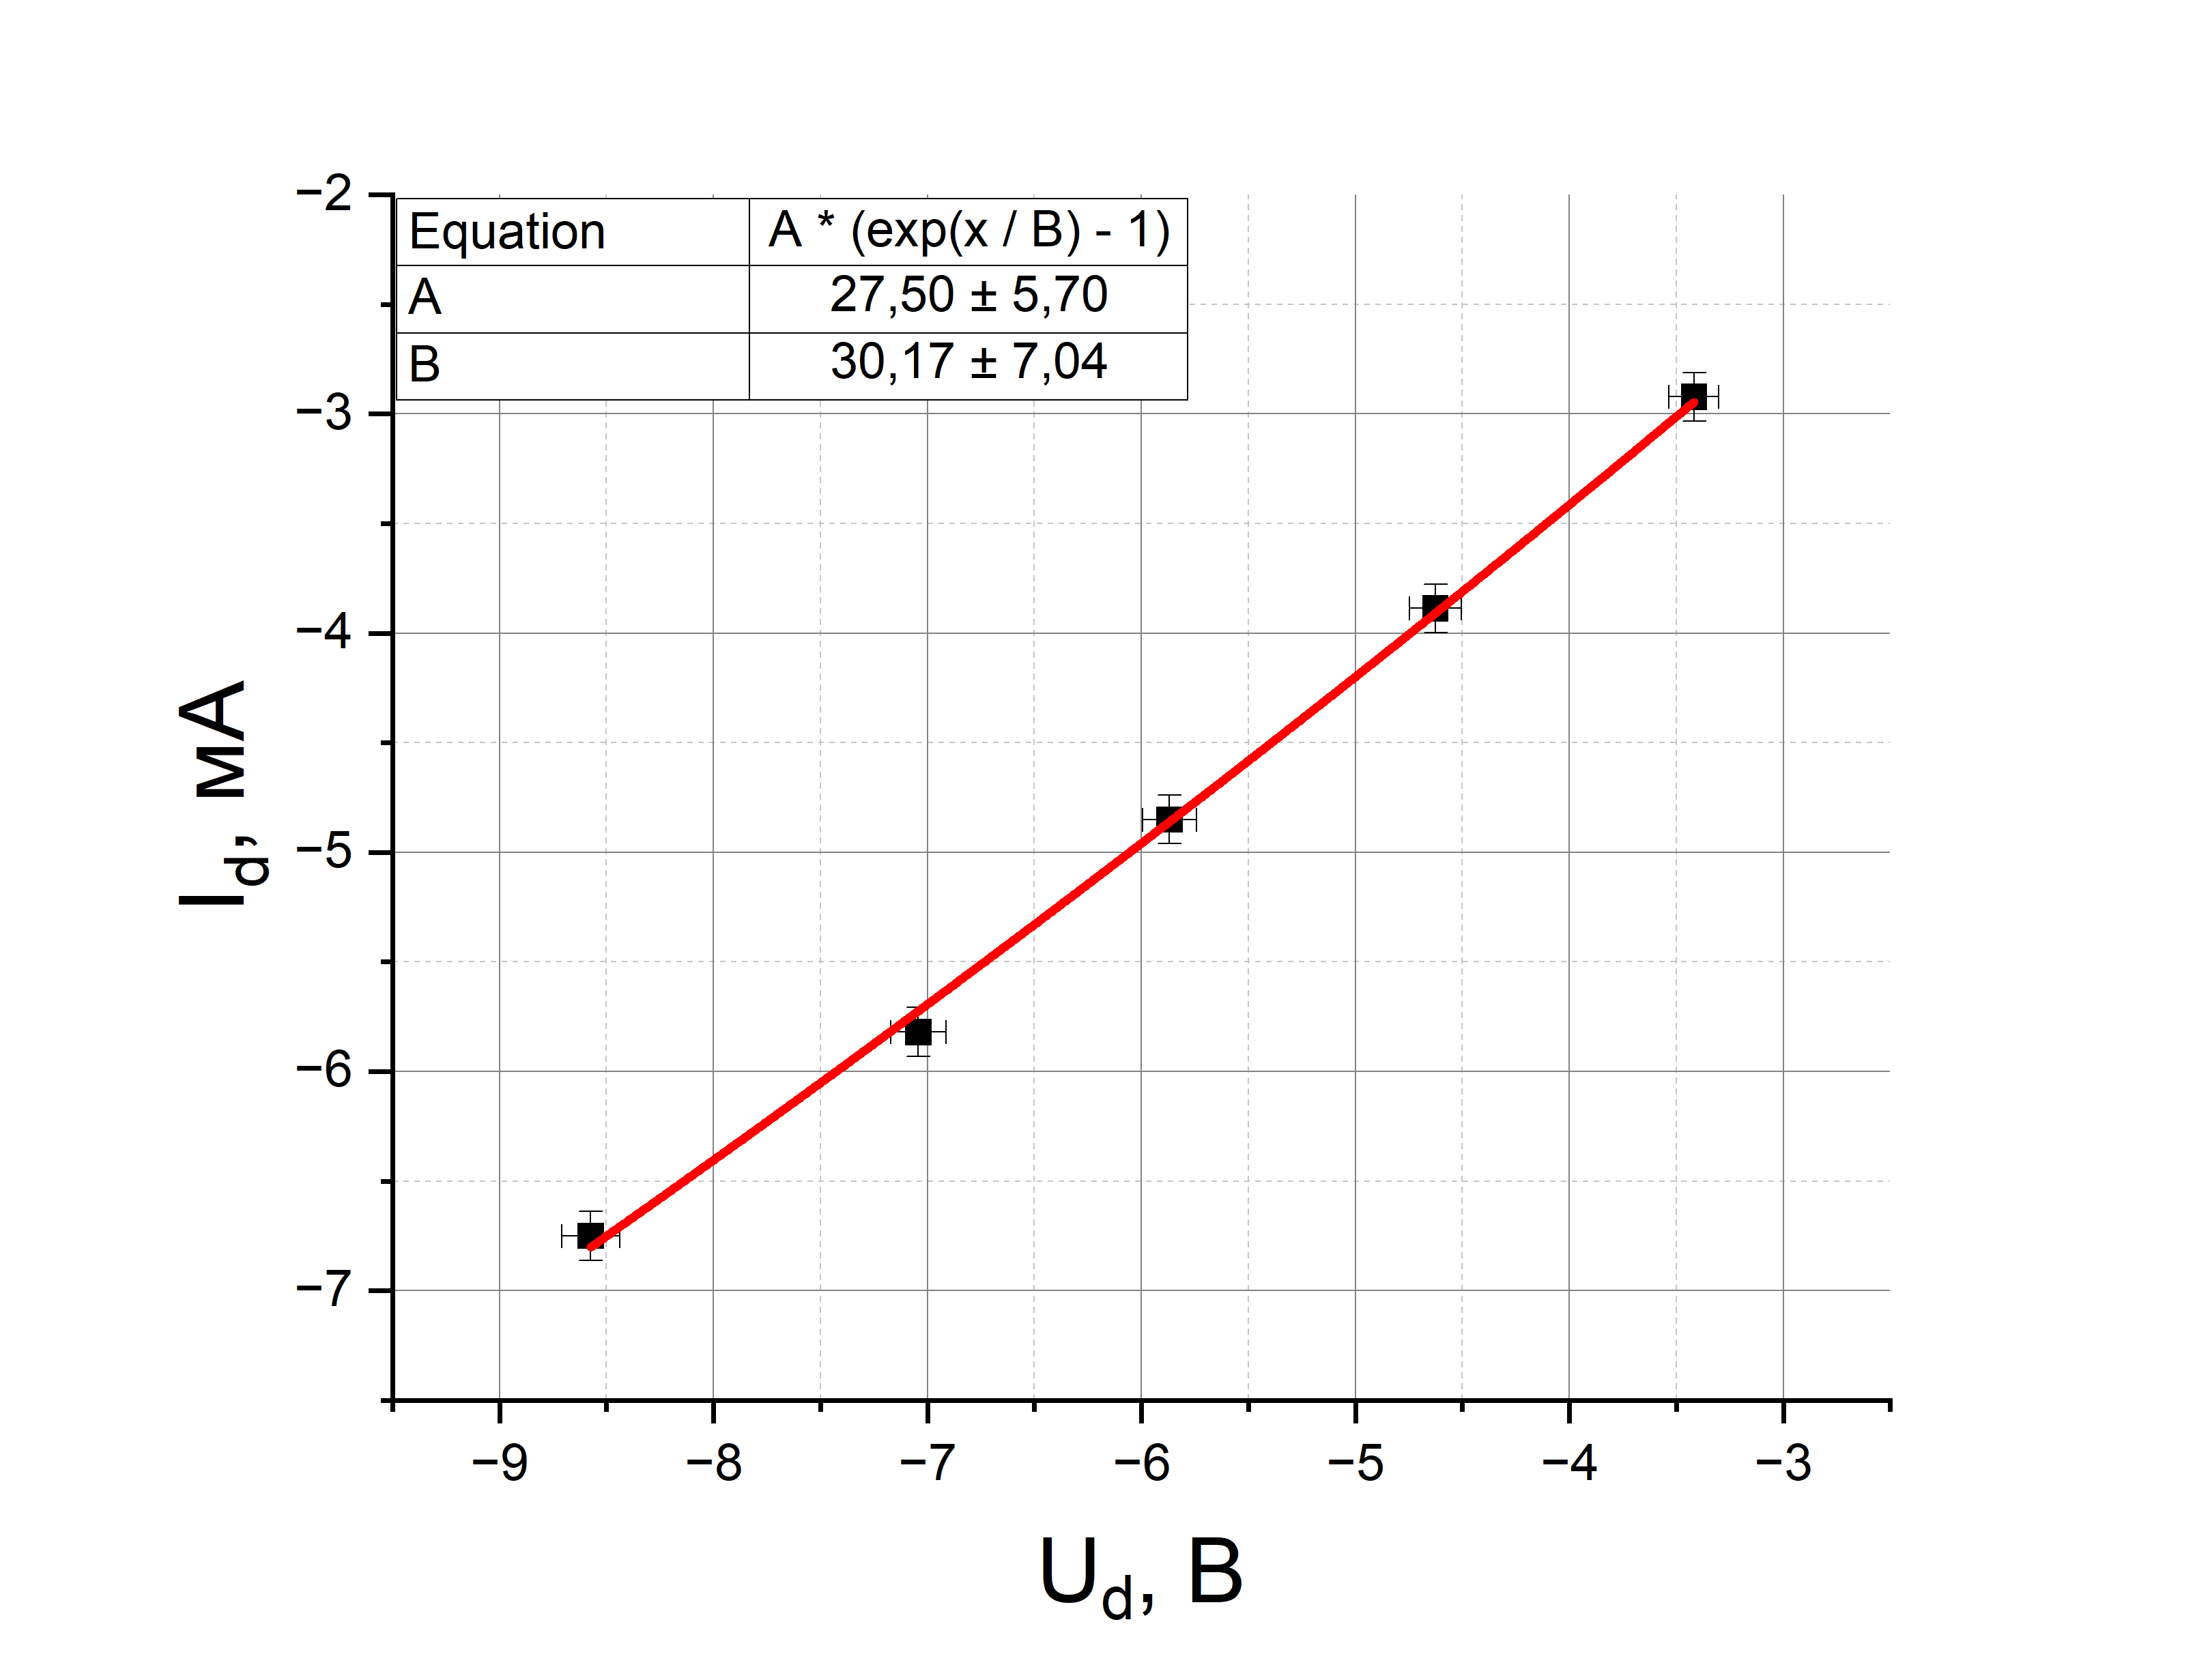
\includegraphics[width=0.8\linewidth]{reverse_T_2}
	\caption{Зависимость тока, протекающего через диод от напряжения на нем при $T \approx 317K$}
\end{figure}

\newpage

\begin{figure}[h!]
	\centering
	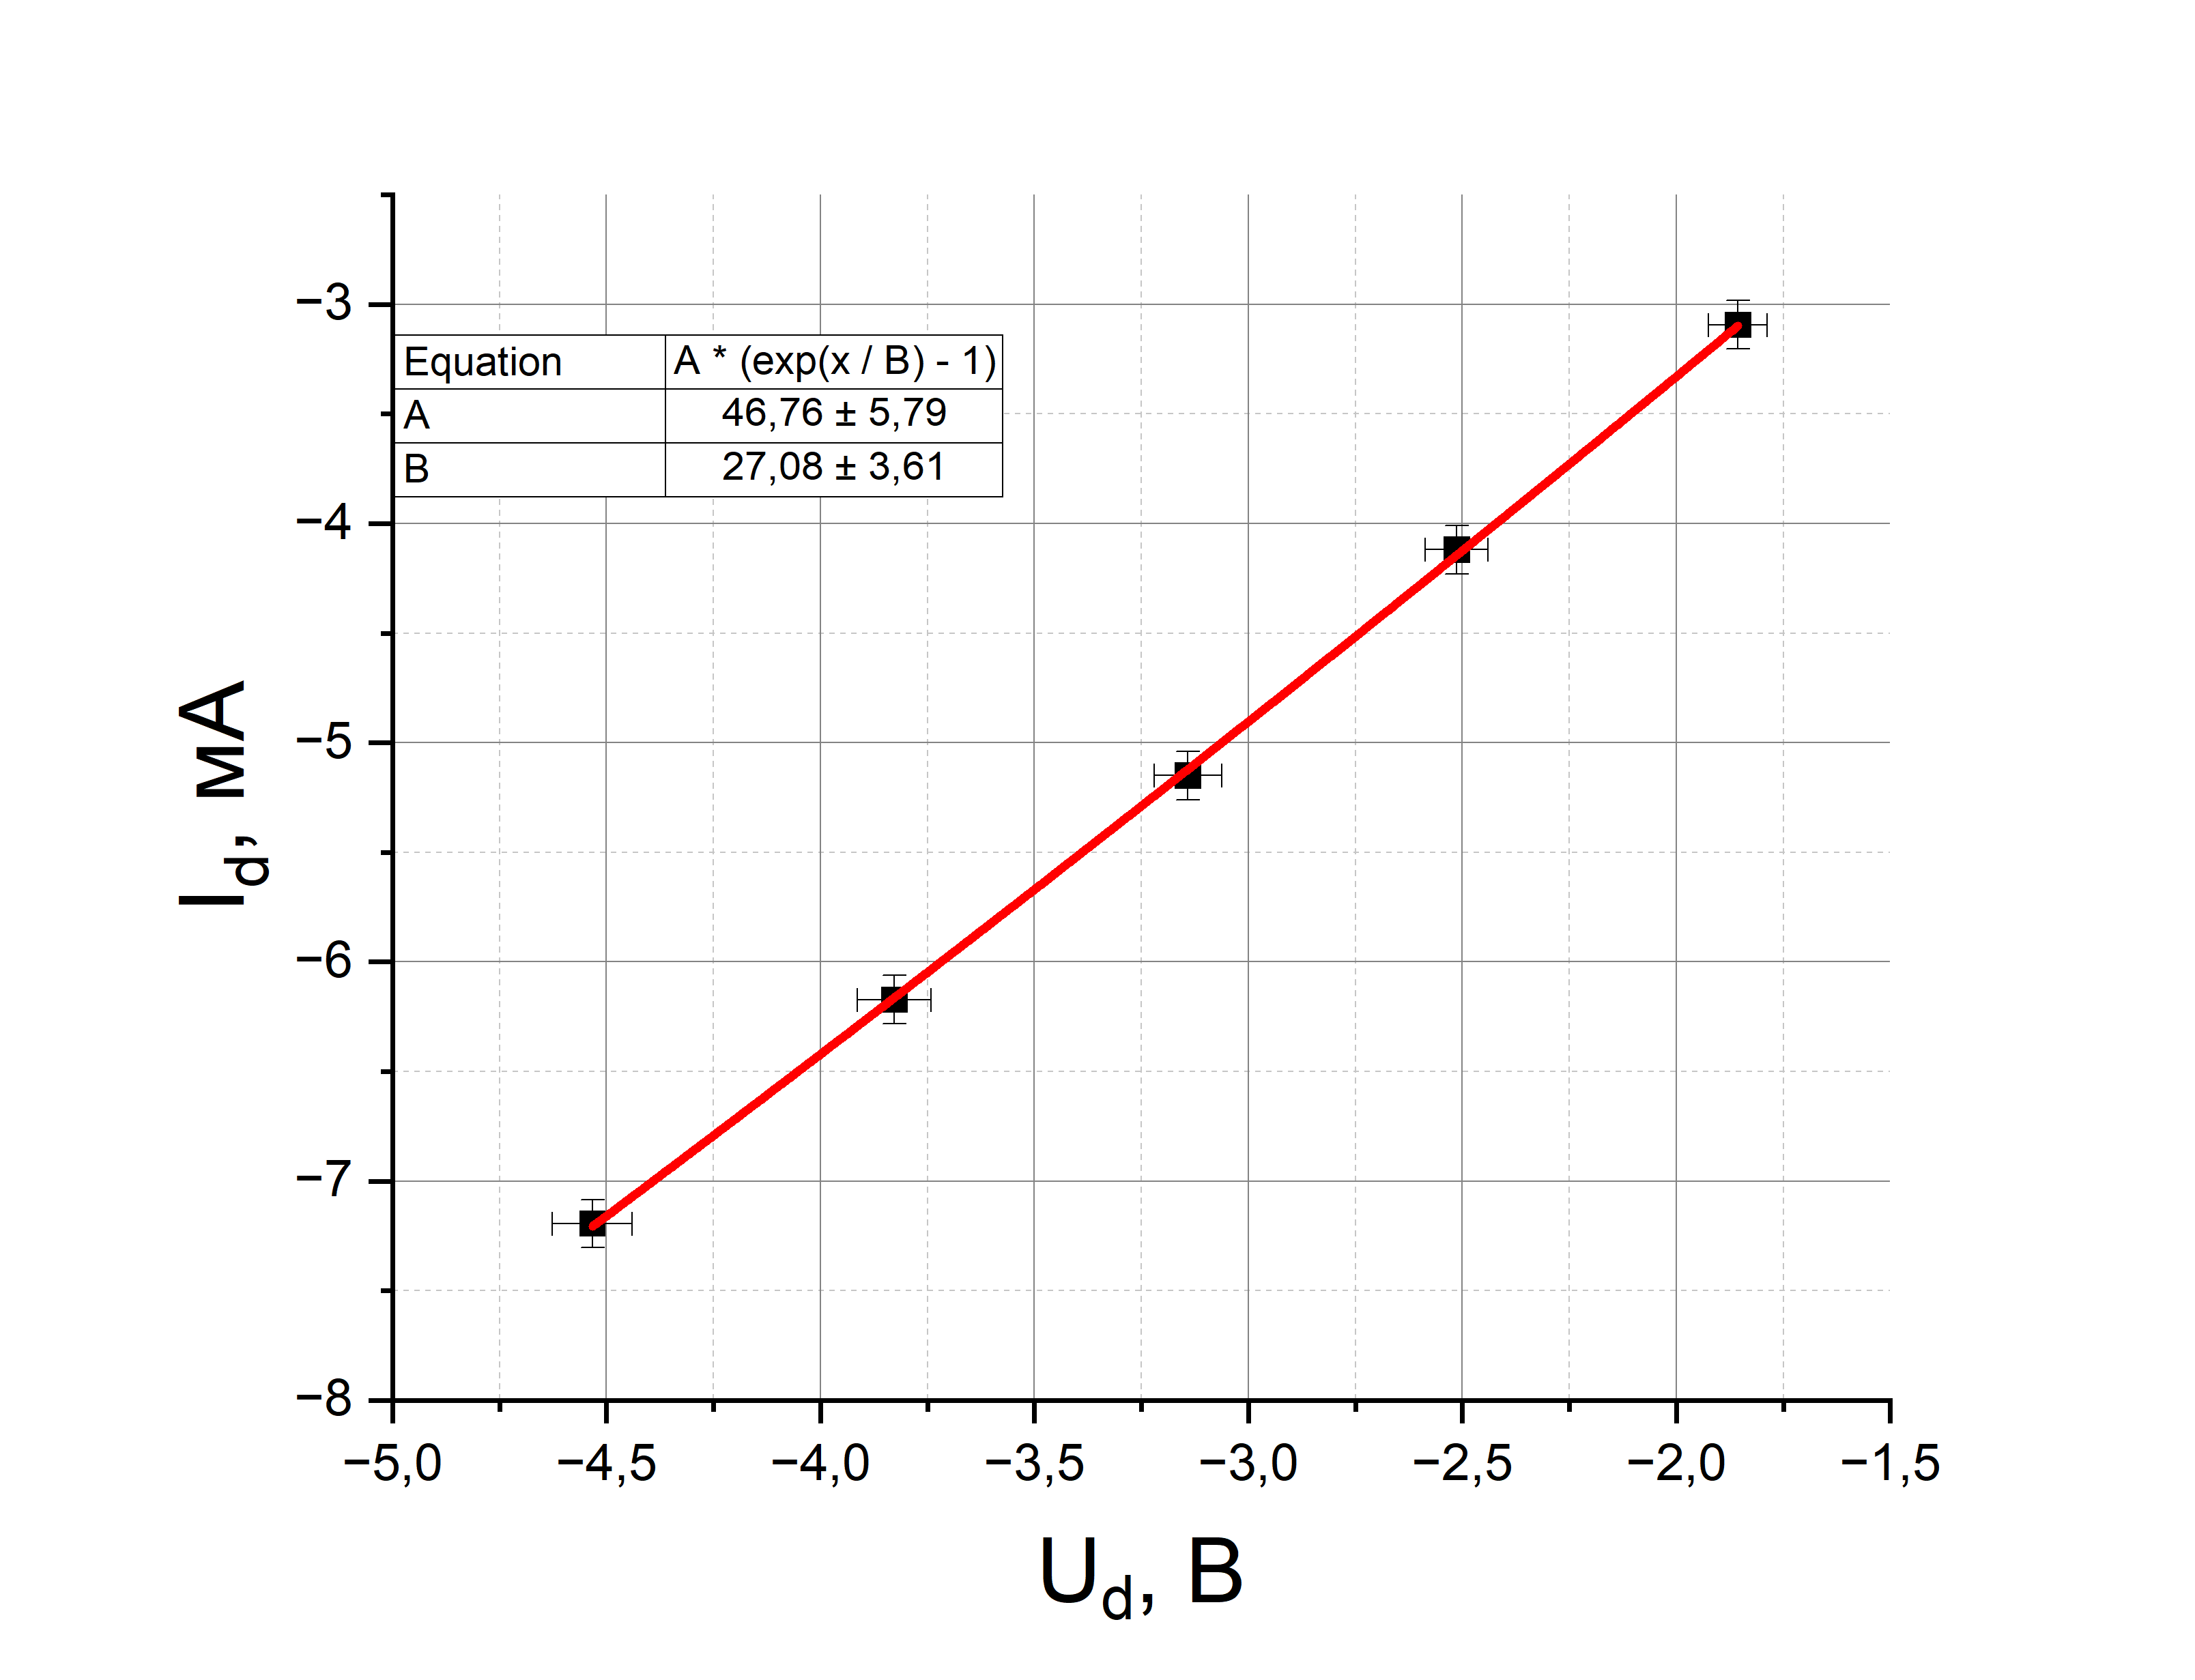
\includegraphics[width=0.8\linewidth]{reverse_T_3}
	\caption{Зависимость тока, протекающего через диод от напряжения на нем при $T \approx 332K$}
\end{figure}

\begin{figure}[h!]
	\centering
	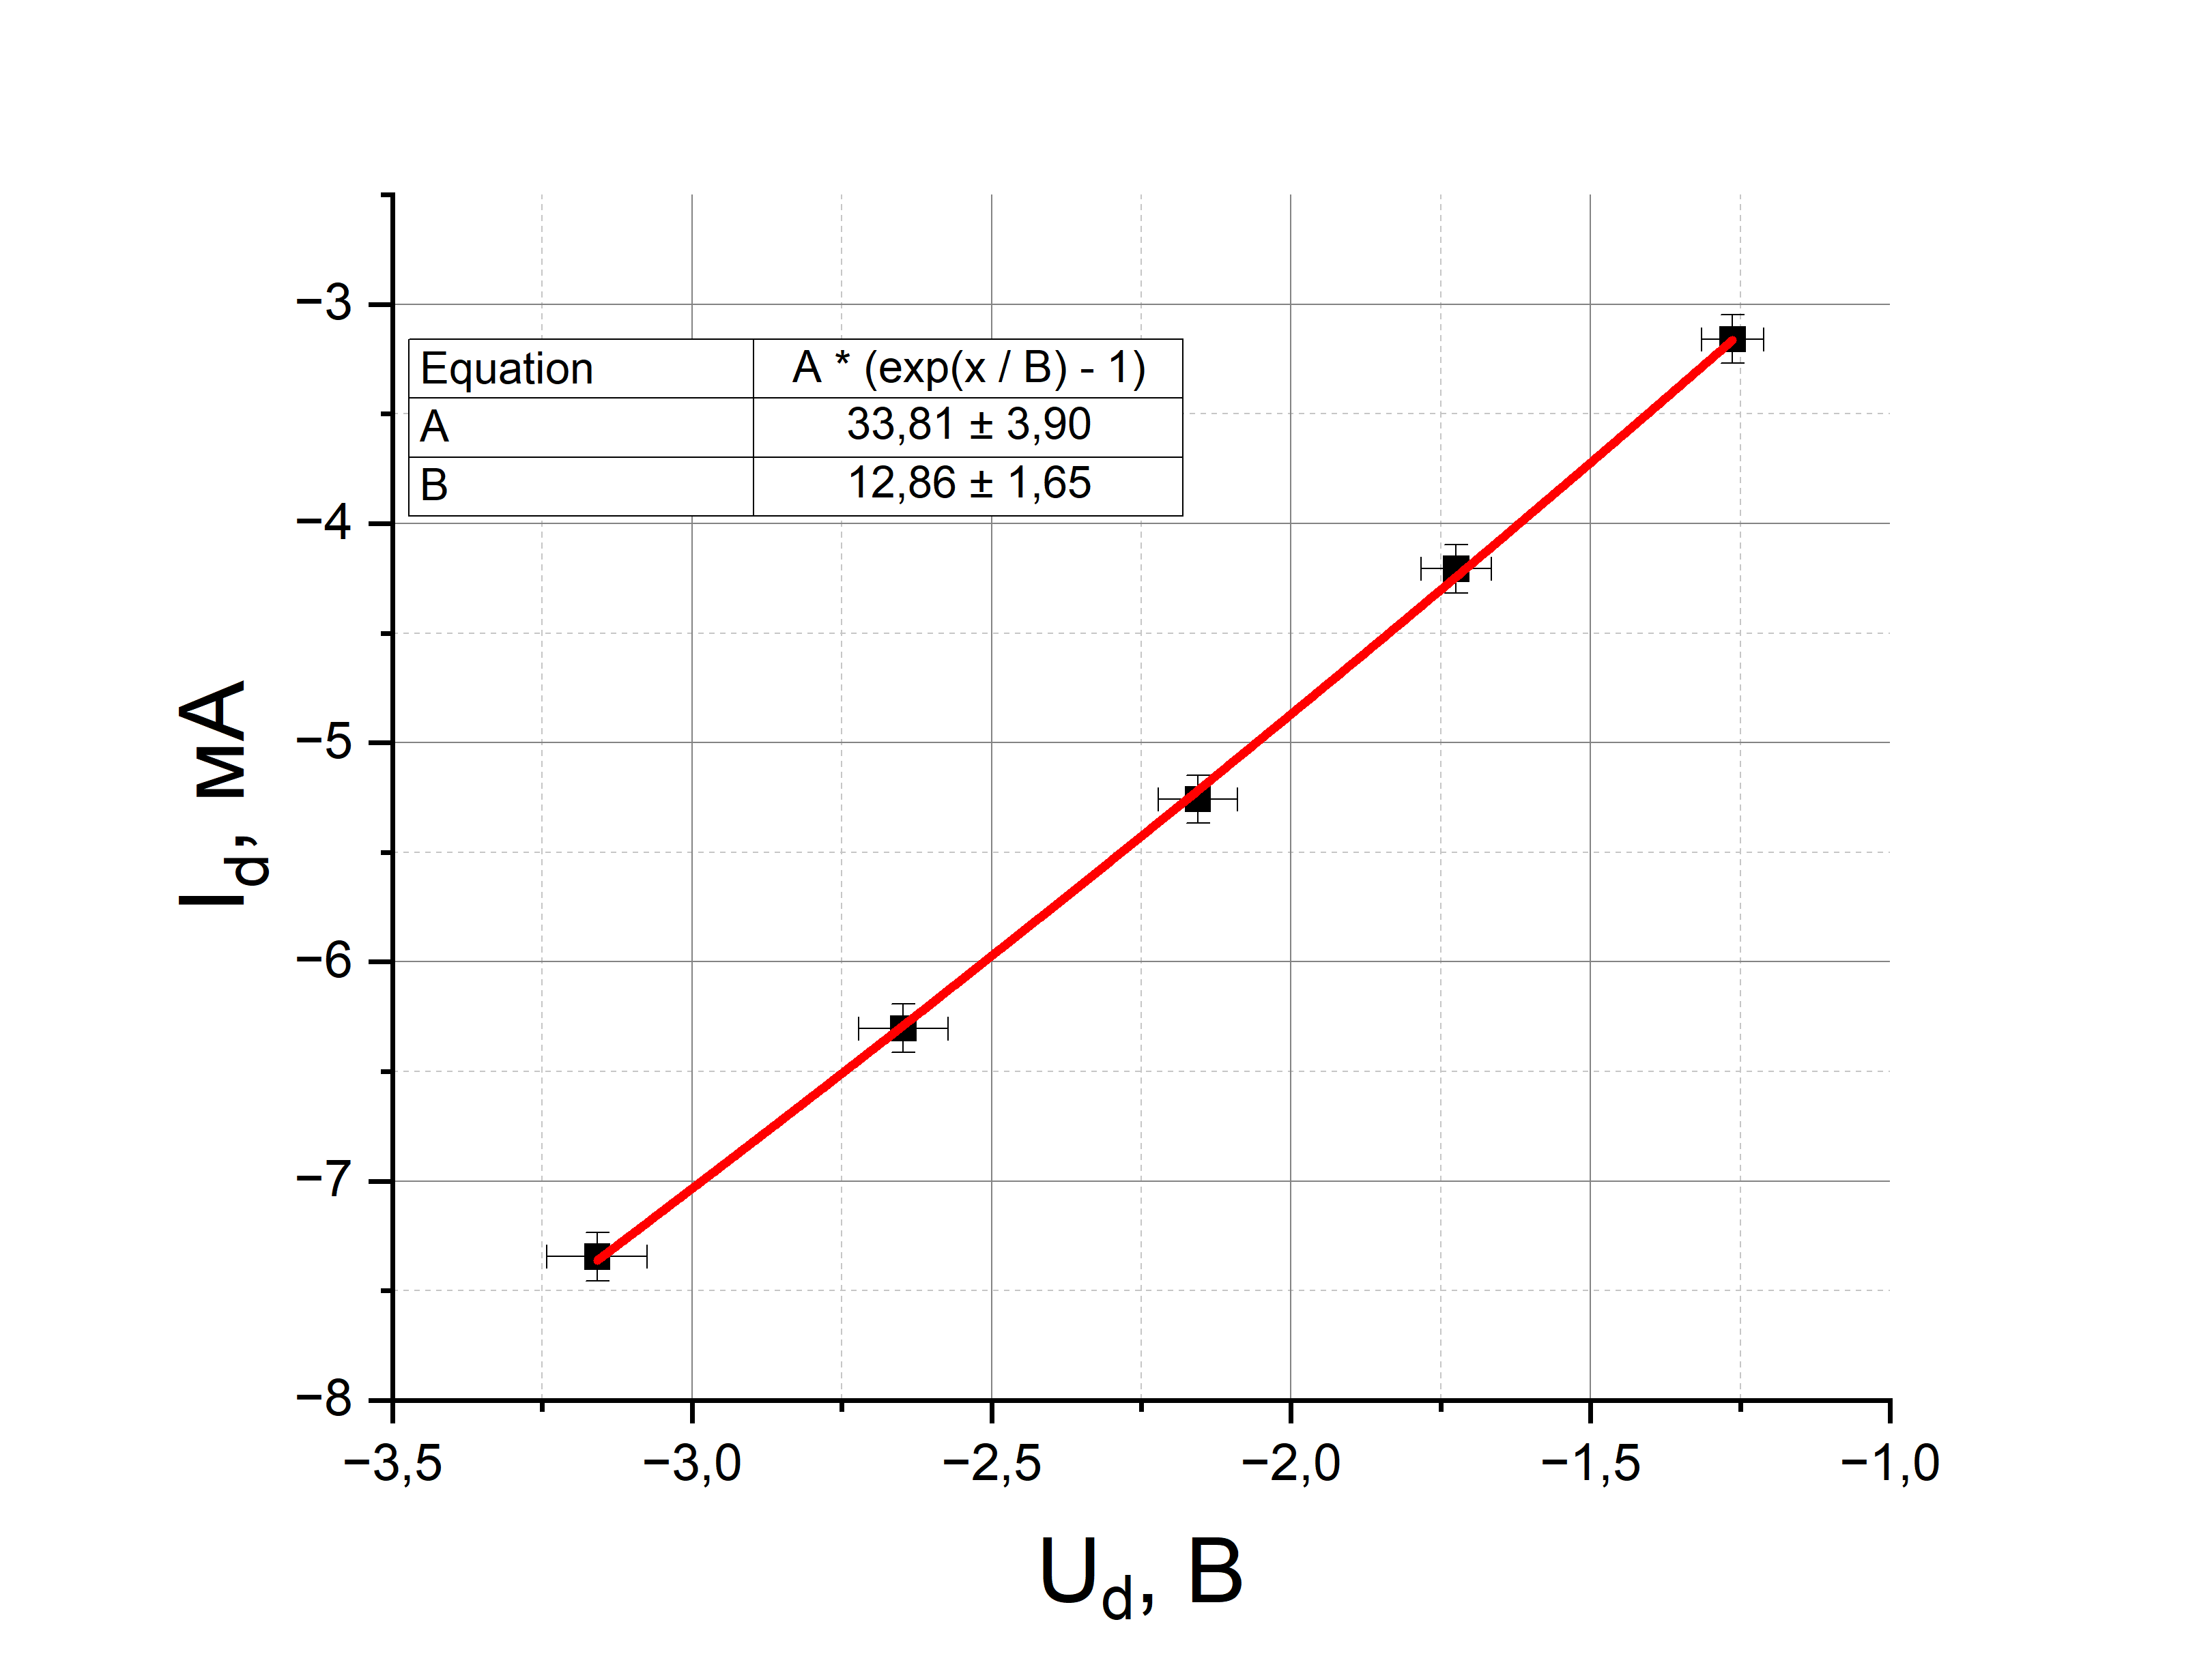
\includegraphics[width=0.8\linewidth]{reverse_T_4}
	\caption{Зависимость тока, протекающего через диод от напряжения на нем при $T \approx 336K$}
\end{figure}

\newpage

Занесем полученные результаты в таблицу:

\begin{table}[h]
\centering
\caption{}
\begin{tabular}{|c|c|c|c|c|}
\hline
$T$, К & 313,86 & 316,95 & 331,48 & 336,24 \\ \hline
$\delta_T$, К & 1,03 & 1,03 & 1,03 & 1,03 \\ \hline
$I_0$, мА & 17,21 & 27,50 & 46,76 & 33,81 \\ \hline
$\delta_{I_0}$, мА & 1,38 & 5,70 & 5,79 & 3,90 \\ \hline
$1/T \cdot 10^3$, К & 3,19 & 3,16 & 3,02 & 2,97 \\ \hline
$\delta 1/T \cdot 10^3$, К & 0,01 & 0,01 & 0,01 & 0,01 \\ \hline
$\ln(I_0/I_1)$ & 2,85 & 3,31 & 3,85 & 3,52 \\ \hline
$\delta_{\ln(I_0/I_1)}$ & 0,08 & 0,21 & 0,12 & 0,12 \\ \hline
\end{tabular}
\end{table}

где $I_1 = 1 мА$, а погрешности рассчитывались по формулам:
\begin{align*}
	\delta_{1/T} &= \frac{\delta_T}{T^2} \\
	\delta_{\ln(I_0/I_1)} &= \frac{\delta_{I_0}}{I_0} \\
\end{align*}

Построим график зависимости $\ln (I_0/I_1) = f(1/T)$:

\begin{figure}[h!]
	\centering
	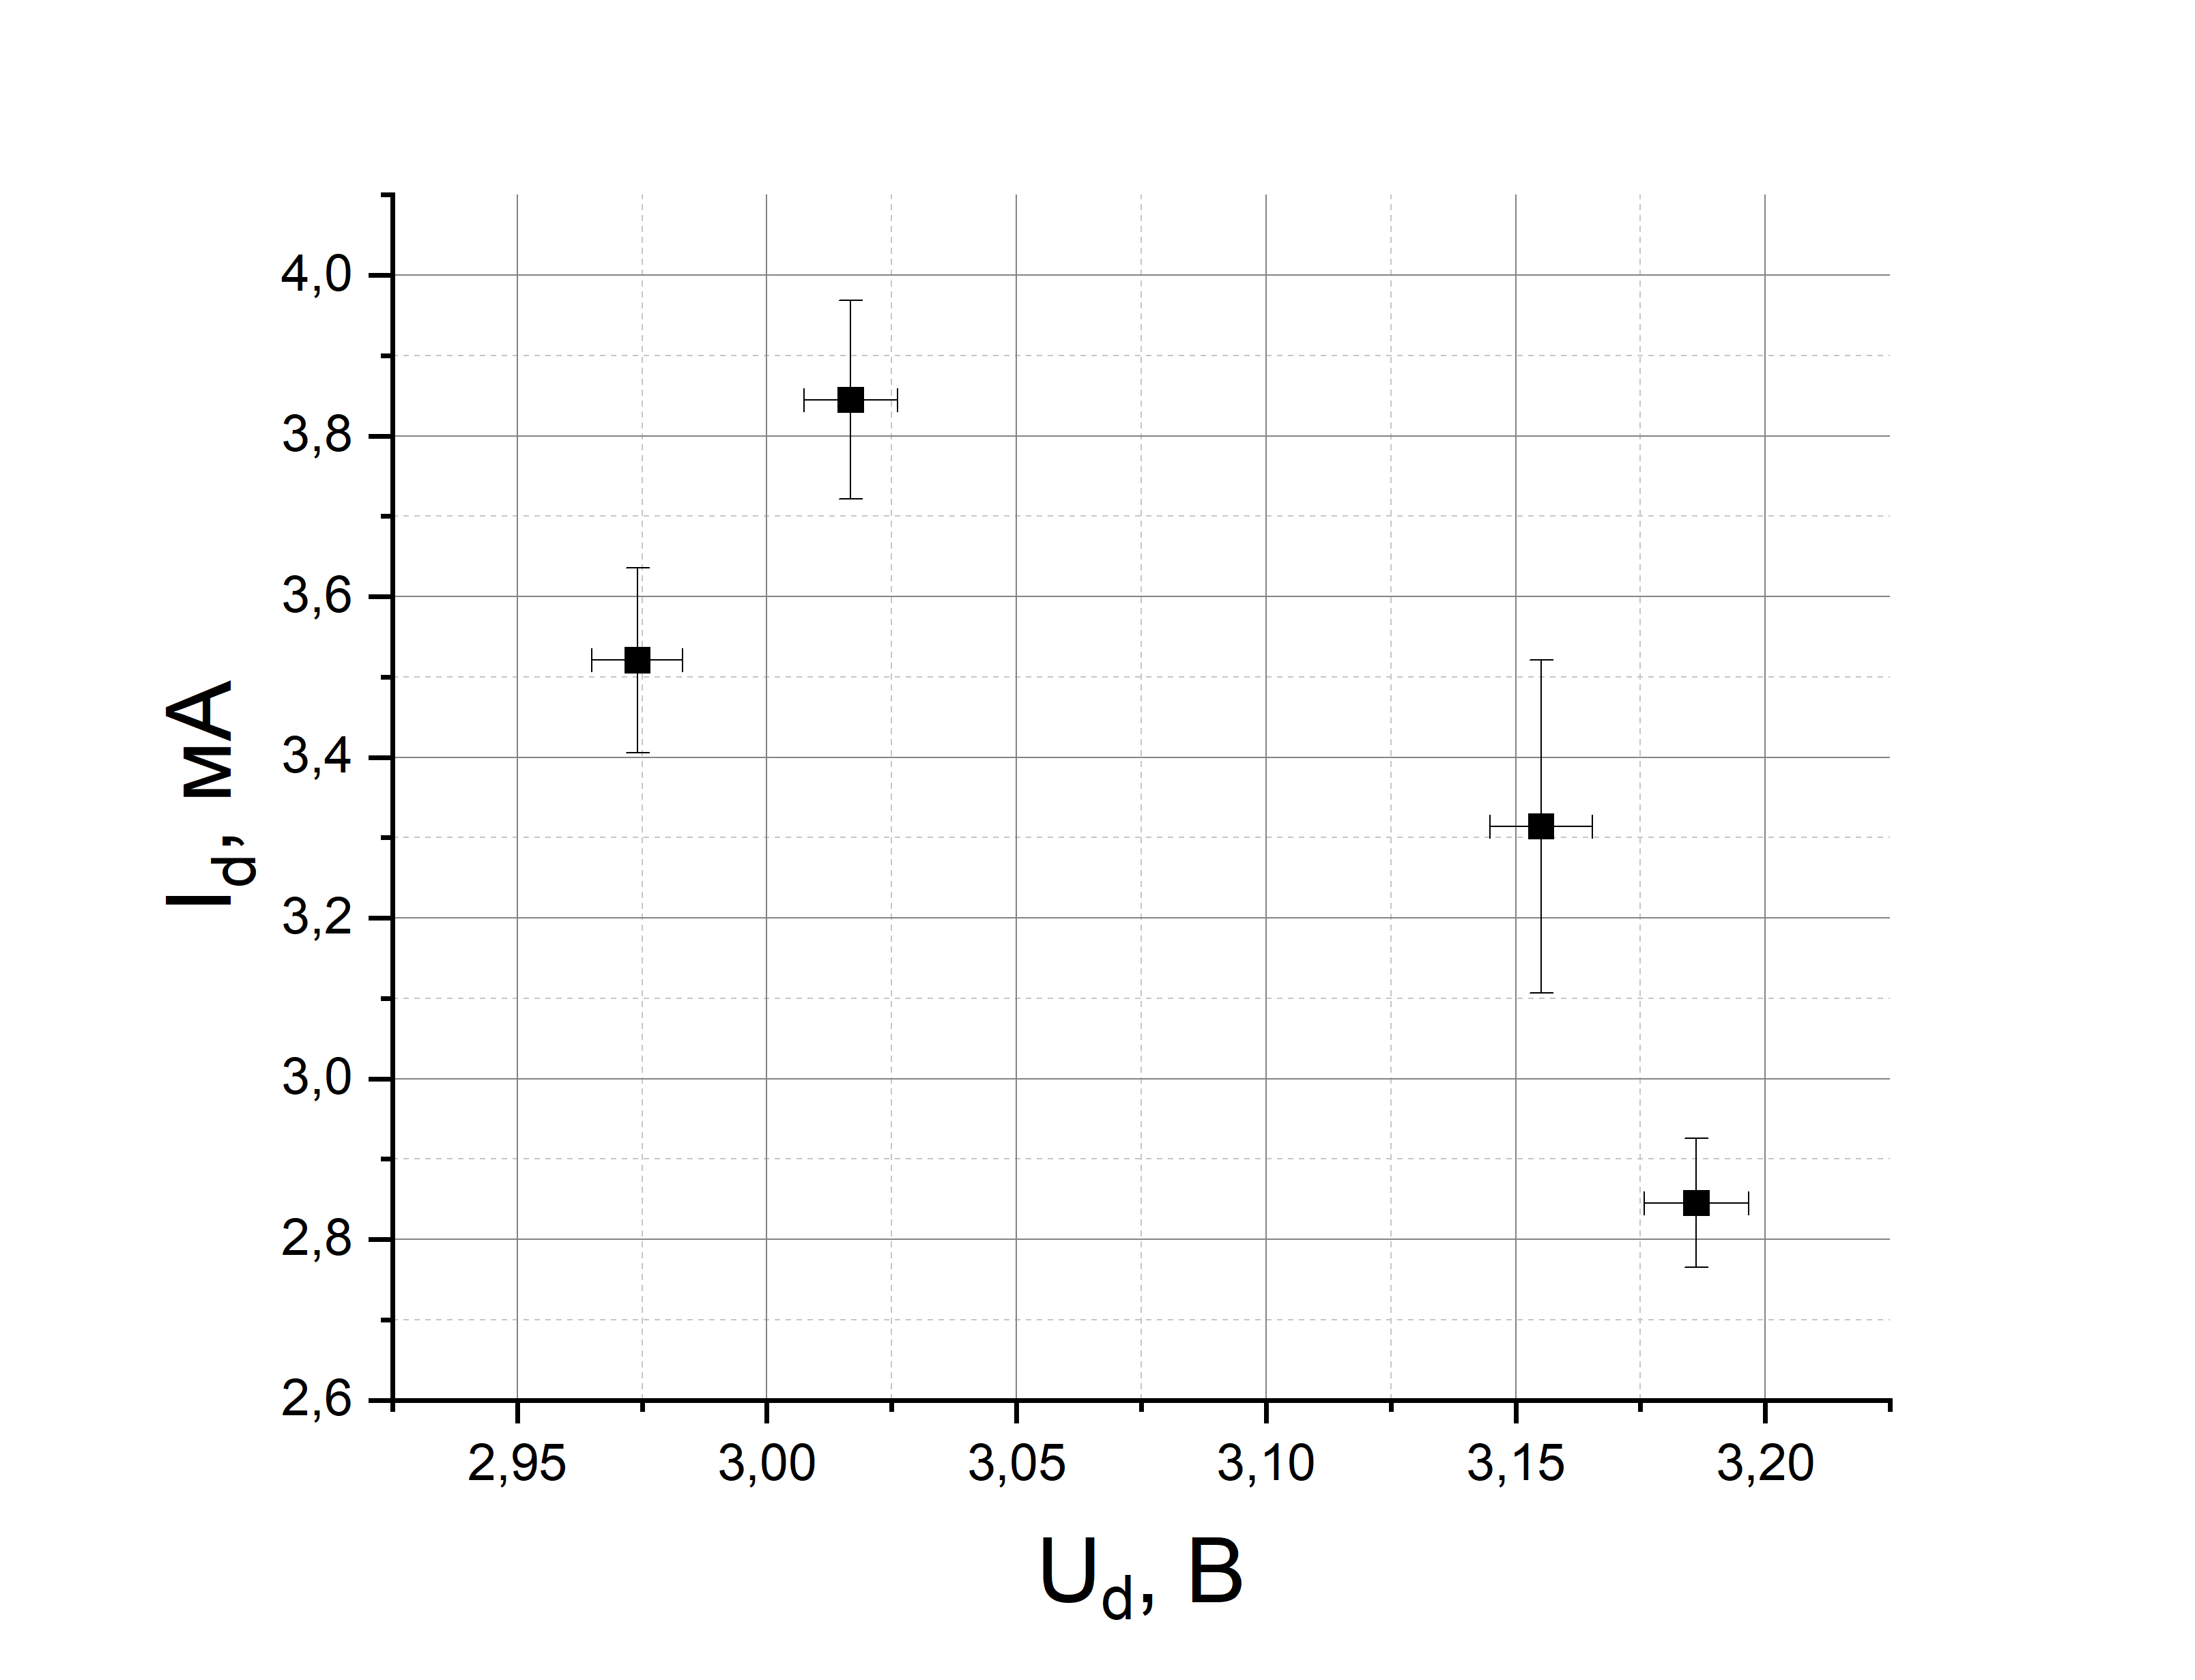
\includegraphics[width=0.8\linewidth]{reverse_current}
	\caption{Зависимость логарифма тока насыщения от обратной температуры}
\end{figure}

Заметим, что первая точка явно выпадает из линейной зависимости, это может быть связано с неаккуратным измерением при высокой температуре. Откинув первую точку, аппроксимируем точки прямой по методу хи-квадрат:

\newpage

\begin{figure}[h!]
	\centering
	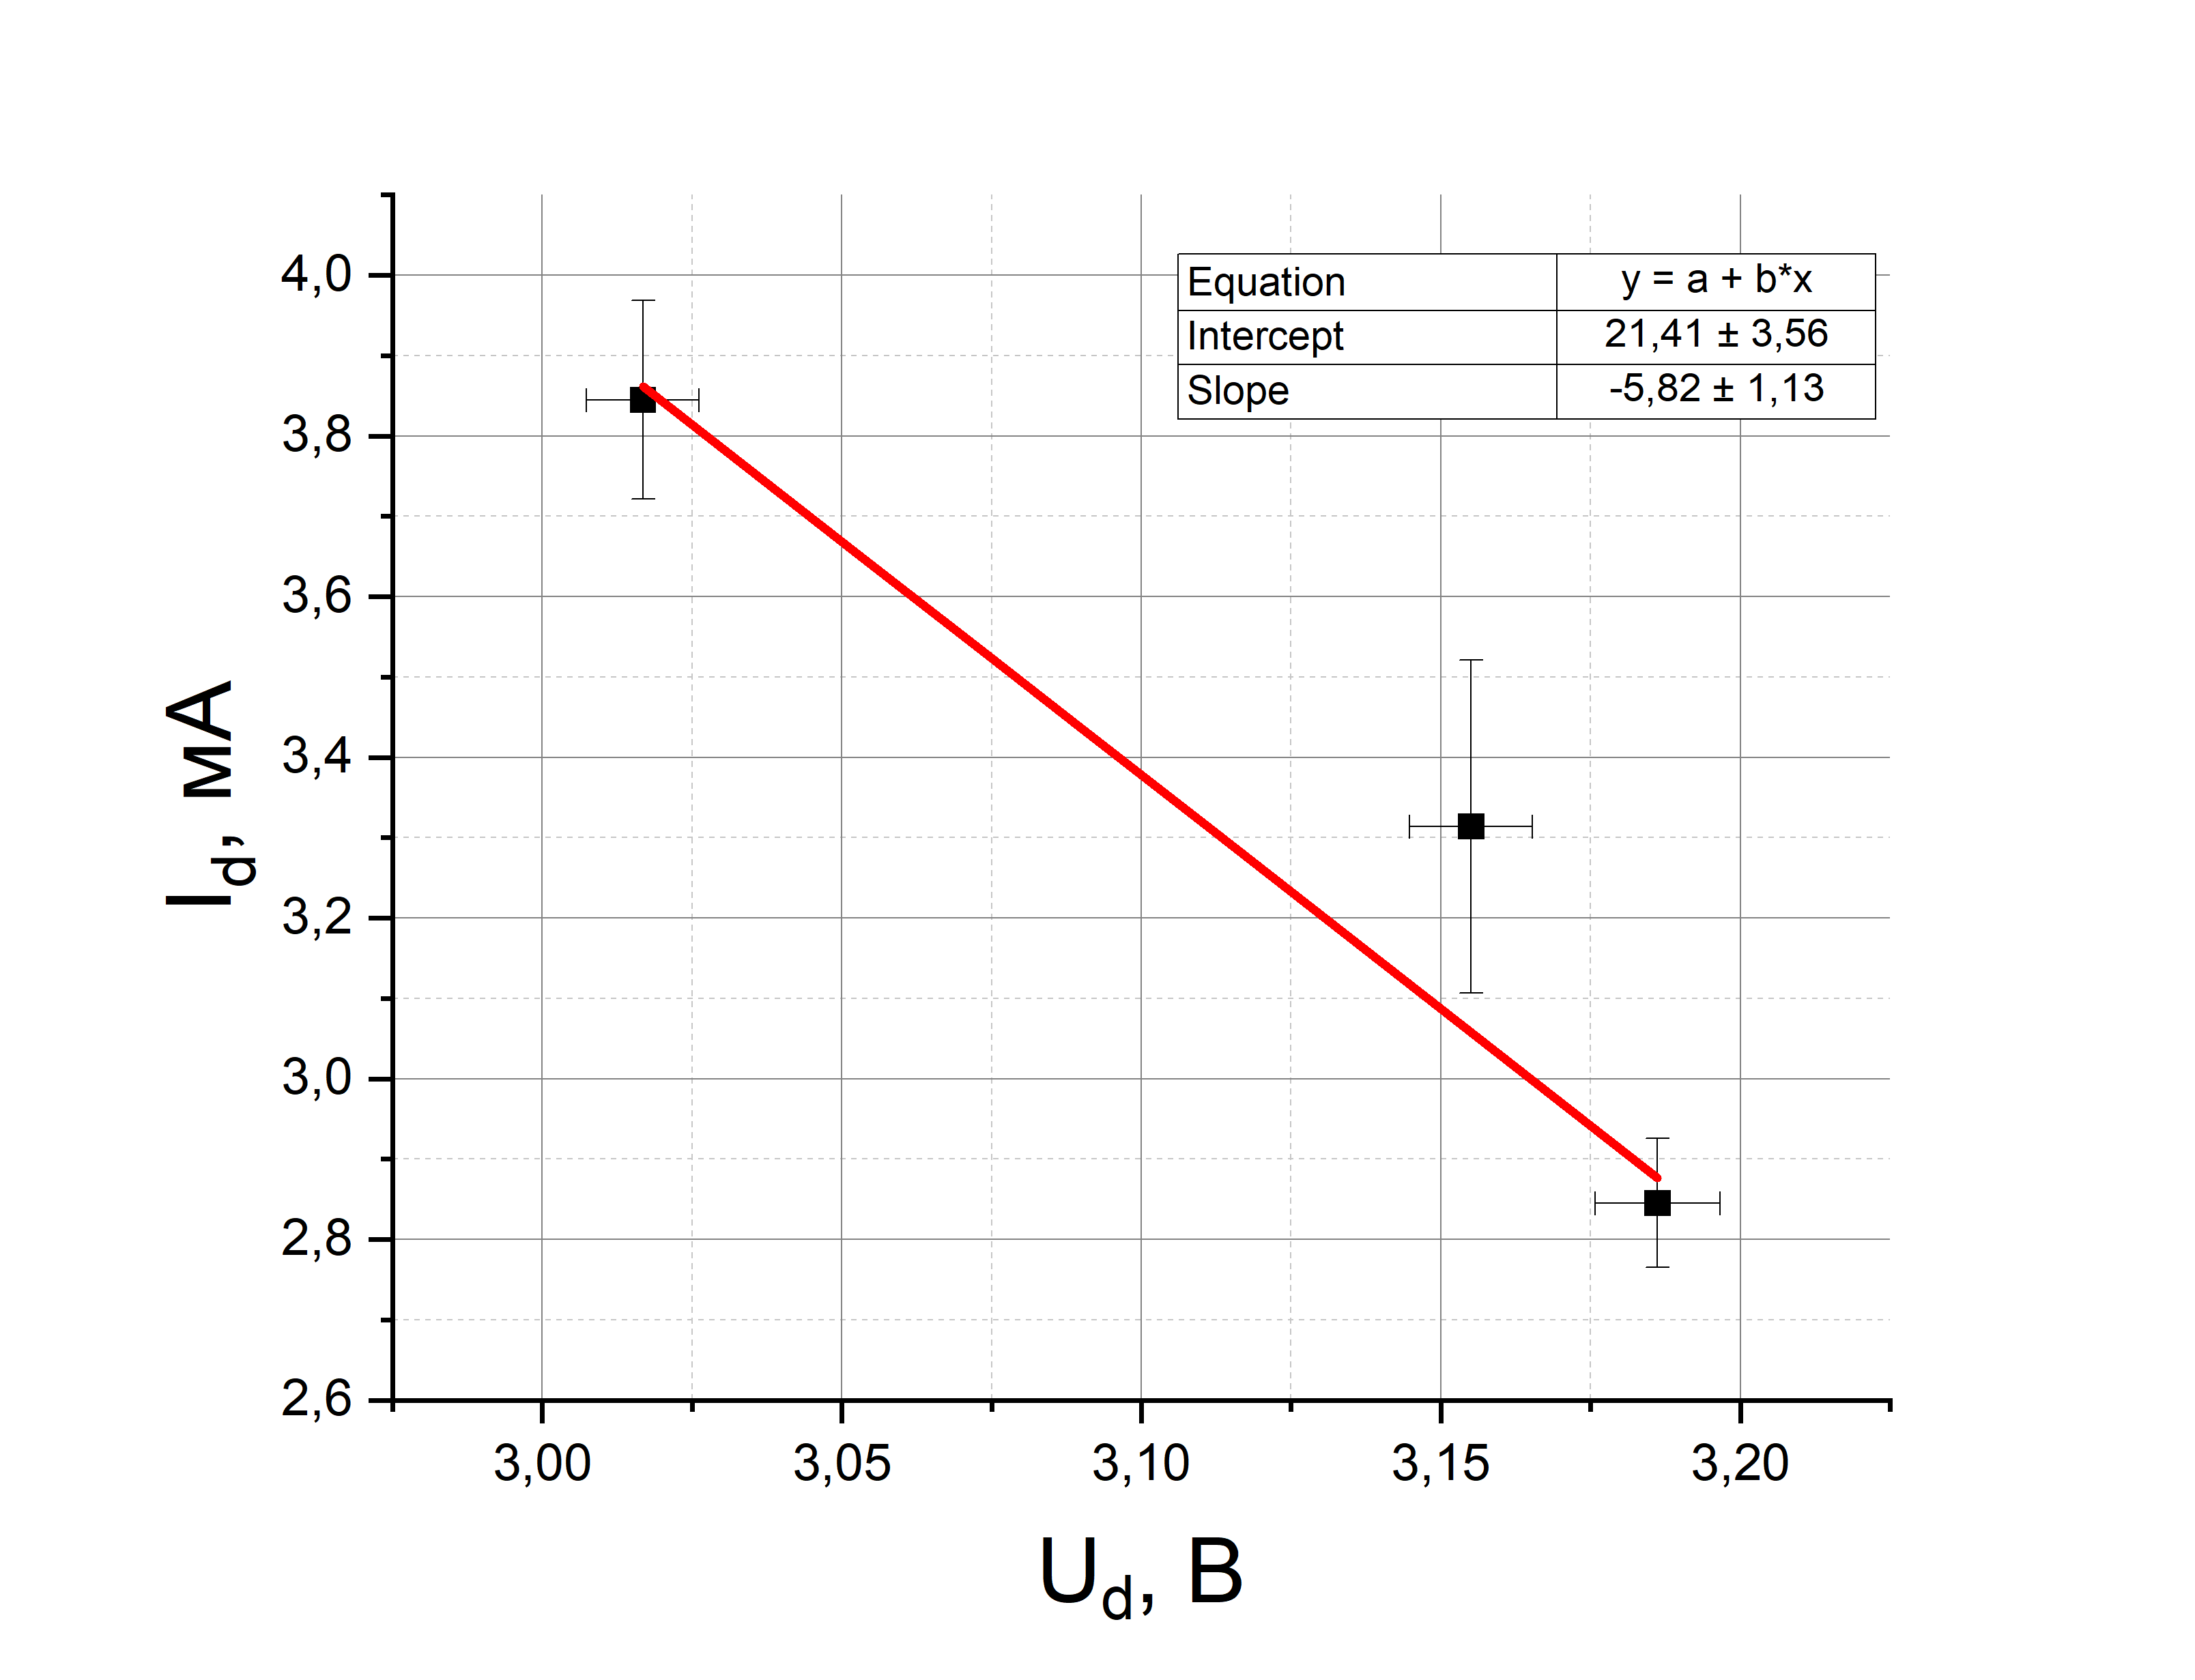
\includegraphics[width=0.7\linewidth]{reverse_current_approx}
	\caption{Зависимость логарифма тока насыщения от обратной температуры}
\end{figure}

Из наклона графика мы можем оценить возникающую контактную разность потенциалов:

$$
	\Delta V = -\frac{k_Б}{e} b = (0.50 \pm 0.09) В
$$

\section*{Определение емкости p-n перехода}

Область перераспределенной зарядовой плотности на p-n переходе может быть рассмотрена как конденсатор с некоторой емкостью. Таким образом, прямоугольный сигнал на диоде будет <<сглаживаться>>, по масштабу сглаживания можно оценить ёмкость (p-n)--перехода

\begin{figure}[h!]
	\centering
	\includegraphics[width=0.6\linewidth]{capacity}
	\caption{Осциллограмма сигнала с диода}
\end{figure}

\newpage

Тогда постоянная времени:

$$
	\tau \approx \frac{2,5}{5} \cdot 10^{-4} = 50 мкс
$$

А емкость (p-n)--перехода:

$$
	C = \frac{\tau}{R_м} = \frac{50}{500} = 0.1 мкФ = 100 нФ
$$

Проанализируем результат. Полная емкость (p-n)--перехода складывается из барьерной и диффузионной емкости. Барьерная емкость обусловлена нескомпенсированным зарядом, сосредоточенным по обе стороны от границы перехода и составляет десятки-сотни пикофарад. Диффузионная емкость возникает при приложении напряжения в прямом направлении, для которого характерно накопление неосновных носителей заряда, причем  $С_{диф} \propto \exp \left( \frac{eU}{k_Б T} \right)$, приведем график зависимости диффузионной емкости от приложенного напряжения:

\begin{figure}[h!]
	\centering
	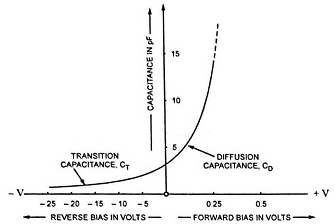
\includegraphics[width=0.5\linewidth]{capacitance}
	\caption{Зависимость емкости (p-n)--перехода от приложенного напряжения}
\end{figure} 

Таким образом, учитывая экспоненциальную зависимость, характерные значения емкости из графика и величину прикладываемого напряжения $V \sim 10 В$ можно предположить, что полученная емкость согласуется с теорией.

\section*{Выводы}
В ходе работы были получены основные параметры выпрямительного диода:
\begin{itemize}
	\item Была измерена контактная разность потенциалов двумя разными методами -- $\Delta V_1 = \linebreak =0,59 \pm 0,02 \ В$ -- по температурной зависимости сопротивления, $\ \Delta V_2 = (0.50 \pm 0.09) \ В$ -- по температурной зависимости обратного тока. Заметим, что метод измерения по температурной зависимости обратного тока является менее точным, так как измерения необходимо было делать быстро, чтобы температура образца сильно не изменилась.
	\item Была получена вольт-амперная характеристика диода при комнатной температуре, с помощью нее были оценены ток насыщения $I_d = (10,64 \pm 0,17) мА$ и параметр неидеальности диода $\theta = 1,50 \pm 0,02$
	\item Также была проанализирована теория емкости (p-n)--перехода и оценена емкость изучаемого диода $C = 100 \ нФ$
\end{itemize}

\end{document}